\onecolumn
\appendices

\section{LLM prompts used in query preprocessing stage}
\label{app:query_preproc_and_aggr_prompts}

Used LLM prompts for different tasks solving in query preprocessing and answer aggregation stages (of QA pipeline) are presented in the following tables:
\begin{itemize}
    \item Table~\ref{tab:qp_denois_gcheck} contains prompts for checking given text fragment on grammatical, syntactical and punctuational errors and reformulate it according to language rules.
    \item Table~\ref{tab:qp_denois_stremov} contains prompts for removing noisy and unnecessary phrases/words from a given text fragment.
    \item Table~\ref{tab:qp_ench_lcheck} contains prompts for editing given text fragment according to grammatical rules.
    \item Table~\ref{tab:qp_ench_tcheck} contains prompts for rephrasing given text fragment with use of commonly used and precise terminology.
    \item Table~\ref{tab:qp_ench_qexp} contains prompts for rephrasing/expanding given text fragment (with use of common language/text patterns) so its meaning becomes more clear for search engines.
    \item Table~\ref{tab:qp_decomp_cls} contains prompts to determine for a given user question: whether it contains several independent sub questions or not.
    \item Table~\ref{tab:qp_decomp_exec} contains prompts for decomposition of a given complex question into several sub questions that can be answered independently to each other.
\end{itemize}
    
\begin{table}[H]
	\renewcommand{\arraystretch}{1.5}
	\centering
	\resizebox{\textwidth}{!}{%
		\begin{tabular}{|c|l|}
			\hline
			\textbf{Type} & \multicolumn{1}{c|}{\textbf{Prompt}} \\ \hline \hline
			\multirow{1}{*}{System} & 
			\begin{minipage}{\textwidth}
				
\includegraphics[clip,trim={.02\textwidth} {.82\textheight} {.03\textwidth} 0mm, width=\textwidth,valign=b]{images/prompts/query_preprop/denoising/grammar_checking/system.pdf}
			\end{minipage}
			\\ \hline
			
			\multirow{1}{*}{User} & 
			\begin{minipage}{\textwidth}
				
\includegraphics[clip,trim={.02\textwidth} {1.2\textheight} {.03\textwidth} 0mm, width=\textwidth,valign=b]{images/prompts/query_preprop/denoising/grammar_checking/user.pdf}
			\end{minipage}
			\\ \hline
			
			\multirow{1}{*}{Assistant} & 
			\begin{minipage}{\textwidth}
				
\includegraphics[clip,trim={.02\textwidth} {1.2\textheight} {.03\textwidth} 0mm, width=\textwidth,valign=b]{images/prompts/query_preprop/denoising/grammar_checking/assistant.pdf}
			\end{minipage}
			\\ \hline
		\end{tabular}%
	}
	\caption{LLM prompts for checking given text fragment on grammatical, syntactical and punctuational errors and reformulating it according to language rules}
	\label{tab:qp_denois_gcheck}
\end{table}

\begin{table}[H]
	\renewcommand{\arraystretch}{1.5}
	\centering
	\resizebox{\textwidth}{!}{%
		\begin{tabular}{|c|l|}
			\hline
			\textbf{Type} & \multicolumn{1}{c|}{\textbf{Prompt}} \\ \hline \hline
			\multirow{1}{*}{System} & 
			\begin{minipage}{\textwidth}
				
\includegraphics[clip,trim={.02\textwidth} {.84\textheight} {.03\textwidth} 0mm, width=\textwidth,valign=b]{images/prompts/query_preprop/denoising/stopwords_removing/system.pdf}
			\end{minipage}
			\\ \hline
			
			\multirow{1}{*}{User} & 
			\begin{minipage}{\textwidth}
				
\includegraphics[clip,trim={.02\textwidth} {1.2\textheight} {.03\textwidth} 0mm, width=\textwidth,valign=b]{images/prompts/query_preprop/denoising/stopwords_removing/user.pdf}
			\end{minipage}
			\\ \hline
			
			\multirow{1}{*}{Assistant} & 
			\begin{minipage}{\textwidth}
				
\includegraphics[clip,trim={.02\textwidth} {1.2\textheight} {.03\textwidth} 0mm, width=\textwidth,valign=b]{images/prompts/query_preprop/denoising/stopwords_removing/assistant.pdf}
			\end{minipage}
			\\ \hline
		\end{tabular}%
	}
	\caption{LLM prompts for removing noisy and unnecessary phrases/words from given text fragment}
	\label{tab:qp_denois_stremov}
\end{table}

\begin{table}[H]
	\renewcommand{\arraystretch}{1.5}
	\centering
	\resizebox{\textwidth}{!}{%
		\begin{tabular}{|c|l|}
			\hline
			\textbf{Type} & \multicolumn{1}{c|}{\textbf{Prompt}} \\ \hline \hline
			\multirow{1}{*}{System} & 
			\begin{minipage}{\textwidth}
				
\includegraphics[clip,trim={.02\textwidth} {1.16\textheight} {.03\textwidth} 0mm, width=\textwidth,valign=b]{images/prompts/query_preprop/enhancing/linguist_check/system.pdf}
			\end{minipage}
			\\ \hline
			
			\multirow{1}{*}{User} & 
			\begin{minipage}{\textwidth}
				
\includegraphics[clip,trim={.02\textwidth} {1.2\textheight} {.03\textwidth} 0mm, width=\textwidth,valign=b]{images/prompts/query_preprop/enhancing/linguist_check/user.pdf}
			\end{minipage}
			\\ \hline
			
			\multirow{1}{*}{Assistant} & 
			\begin{minipage}{\textwidth}
				
\includegraphics[clip,trim={.02\textwidth} {1.2\textheight} {.03\textwidth} 0mm, width=\textwidth,valign=b]{images/prompts/query_preprop/enhancing/linguist_check/assistant.pdf}
			\end{minipage}
			\\ \hline
		\end{tabular}%
	}
	\caption{LLM prompts for editing given text fragment according to grammatical rules}
	\label{tab:qp_ench_lcheck}
\end{table}

\begin{table}[H]
	\renewcommand{\arraystretch}{1.5}
	\centering
	\resizebox{\textwidth}{!}{%
		\begin{tabular}{|c|l|}
			\hline
			\textbf{Type} & \multicolumn{1}{c|}{\textbf{Prompt}} \\ \hline \hline
			\multirow{1}{*}{System} & 
			\begin{minipage}{\textwidth}
				
\includegraphics[clip,trim={.02\textwidth} {.8\textheight} {.03\textwidth} 0mm, width=\textwidth,valign=b]{images/prompts/query_preprop/enhancing/terms_check/system.pdf}
			\end{minipage}
			\\ \hline
			
			\multirow{1}{*}{User} & 
			\begin{minipage}{\textwidth}
				
\includegraphics[clip,trim={.02\textwidth} {1.2\textheight} {.03\textwidth} 0mm, width=\textwidth,valign=b]{images/prompts/query_preprop/enhancing/terms_check/user.pdf}
			\end{minipage}
			\\ \hline
			
			\multirow{1}{*}{Assistant} & 
			\begin{minipage}{\textwidth}
				
\includegraphics[clip,trim={.02\textwidth} {1.2\textheight} {.03\textwidth} 0mm, width=\textwidth,valign=b]{images/prompts/query_preprop/enhancing/terms_check/assistant.pdf}
			\end{minipage}
			\\ \hline
		\end{tabular}%
	}
	\caption{LLM prompts for rephrasing given text fragment with use of commonly used and precise terminology}
	\label{tab:qp_ench_tcheck}
\end{table}

\begin{table}[H]
	\renewcommand{\arraystretch}{1.5}
	\centering
	\resizebox{\textwidth}{!}{%
		\begin{tabular}{|c|l|}
			\hline
			\textbf{Type} & \multicolumn{1}{c|}{\textbf{Prompt}} \\ \hline \hline
			\multirow{1}{*}{System} & 
			\begin{minipage}{\textwidth}
				
\includegraphics[clip,trim={.02\textwidth} {.84\textheight} {.03\textwidth} 0mm, width=\textwidth,valign=b]{images/prompts/query_preprop/enhancing/query_expanstion/system.pdf}
			\end{minipage}
			\\ \hline
			
			\multirow{1}{*}{User} & 
			\begin{minipage}{\textwidth}
				
\includegraphics[clip,trim={.02\textwidth} {1.2\textheight} {.03\textwidth} 0mm, width=\textwidth,valign=b]{images/prompts/query_preprop/enhancing/query_expanstion/user.pdf}
			\end{minipage}
			\\ \hline
			
			\multirow{1}{*}{Assistant} & 
			\begin{minipage}{\textwidth}
				
\includegraphics[clip,trim={.02\textwidth} {1.2\textheight} {.03\textwidth} 0mm, width=\textwidth,valign=b]{images/prompts/query_preprop/enhancing/query_expanstion/assistant.pdf}
			\end{minipage}
			\\ \hline
		\end{tabular}%
	}
	\caption{LLM prompts for rephrasing/expanding given text fragment (with use of common language/text patterns) so its meaning become more clear for search engines}
	\label{tab:qp_ench_qexp}
\end{table}

\begin{table}[H]
	\renewcommand{\arraystretch}{1.5}
	\centering
	\resizebox{\textwidth}{!}{%
		\begin{tabular}{|c|l|}
			\hline
			\textbf{Type} & \multicolumn{1}{c|}{\textbf{Prompt}} \\ \hline \hline
			\multirow{1}{*}{System} & 
			\begin{minipage}{\textwidth}
				
\includegraphics[clip,trim={.02\textwidth} {.42\textheight} {.03\textwidth} 0mm, width=\textwidth,valign=b]{images/prompts/query_preprop/decomposition/decomposition_classifier/system.pdf}
			\end{minipage}
			\\ \hline
			
			\multirow{1}{*}{User} & 
			\begin{minipage}{\textwidth}
				
\includegraphics[clip,trim={.02\textwidth} {1.2\textheight} {.03\textwidth} 0mm, width=\textwidth,valign=b]{images/prompts/query_preprop/decomposition/decomposition_classifier/user.pdf}
			\end{minipage}
			\\ \hline
			
			\multirow{1}{*}{Assistant} & 
			\begin{minipage}{\textwidth}
				
\includegraphics[clip,trim={.02\textwidth} {1.2\textheight} {.03\textwidth} 0mm, width=\textwidth,valign=b]{images/prompts/query_preprop/decomposition/decomposition_classifier/assistant.pdf}
			\end{minipage}
			\\ \hline
		\end{tabular}%
	}
	\caption{LLM prompts to determine for a given user question: whether it contains several independent sub questions or not}
	\label{tab:qp_decomp_cls}
\end{table}

\begin{table}[H]
	\renewcommand{\arraystretch}{1.5}
	\centering
	\resizebox{\textwidth}{!}{%
		\begin{tabular}{|c|l|}
			\hline
			\textbf{Type} & \multicolumn{1}{c|}{\textbf{Prompt}} \\ \hline \hline
			\multirow{1}{*}{System} & 
			\begin{minipage}{\textwidth}
				
\includegraphics[clip,trim={.02\textwidth} {.67\textheight} {.03\textwidth} 0mm, width=\textwidth,valign=b]{images/prompts/query_preprop/decomposition/query_decomposition/system.pdf}
			\end{minipage}
			\\ \hline
			
			\multirow{1}{*}{User} & 
			\begin{minipage}{\textwidth}
				
\includegraphics[clip,trim={.02\textwidth} {1.2\textheight} {.03\textwidth} 0mm, width=\textwidth,valign=b]{images/prompts/query_preprop/decomposition/query_decomposition/user.pdf}
			\end{minipage}
			\\ \hline
			
			\multirow{1}{*}{Assistant} & 
			\begin{minipage}{\textwidth}
				
\includegraphics[clip,trim={.02\textwidth} {1.2\textheight} {.03\textwidth} 0mm, width=\textwidth,valign=b]{images/prompts/query_preprop/decomposition/query_decomposition/assistant.pdf}
			\end{minipage}
			\\ \hline
		\end{tabular}%
	}
	\caption{LLM prompts for decomposition of given complex question into several sub questions, that can be answered independently to each other}
	\label{tab:qp_decomp_exec}
\end{table}


\section{LLM prompts used in proposed memory graph exploration and answer aggregation stages}
\label{app:medium_kg_reasoner_prompts}

Used LLM prompts for different tasks solving in proposed knowledge graph reasoner (in QA pipeline) are presented in the following tables:
\begin{itemize}
    \item Table~\ref{tab:kgreasoner_spenh_pinit} contains prompts for basic search plan generation.
    \item Table~\ref{tab:kgreasoner_entextr_entextr} contains prompts for named entities extraction from a search plan step.
    \item Table~\ref{tab:kgreasoner_clqgen_clqgen} contains prompts for clue-questions generation based on a search plan step and the set of object vertices (from memory graph), associated with that step.
    \item Table~\ref{tab:kgreasoner_clagen_clagen} contains prompts for answer generation on a clue question based on a set of triplets, extracted from memory graph.
    \item Table~\ref{tab:kgreasoner_clagen_summ} contains prompts for clue-answers summarization.
    \item Table~\ref{tab:kgreasoner_answgen_answcls} contains prompts to determine based on the current search plan and the current set of information, extracted from memory, whether it is possible to generate an answer to the user question or not.
    \item Table~\ref{tab:kgreasoner_answgen_answgen} contains prompts for final answer generation to the user question.
    \item Table~\ref{tab:kgreasoner_spenh_enchcls} contains prompts to determine for a given search plan whether it needs to be regenerated/enhanced (based on obtained information from previous steps) or not.
    \item Table~\ref{tab:kgreasoner_spenh_planench} contains prompts to enhance uncompleted search plan steps, taking into account information, extracted from memory on previous steps.
    \item Table~\ref{tab:aggr_answ_summ} contains prompts for answer generation to user question based on sub-answers of its sub-questions.
\end{itemize}

\begin{table}[H]
	\renewcommand{\arraystretch}{1.5}
	\centering
	\resizebox{\textwidth}{!}{%
		\begin{tabular}{|c|l|}
			\hline
			\textbf{Type} & \multicolumn{1}{c|}{\textbf{Prompt}} \\ \hline \hline
			\multirow{1}{*}{System} & 
			\begin{minipage}{\textwidth}
				
\includegraphics[clip,trim={.02\textwidth} {.44\textheight} {.03\textwidth} 0mm, width=\textwidth,valign=b]{images/prompts/medium_reasoner/searchplan_enhancer/plan_initializer/system.pdf}
			\end{minipage}
			\\ \hline
			
			\multirow{1}{*}{User} & 
			\begin{minipage}{\textwidth}
				
\includegraphics[clip,trim={.02\textwidth} {1.2\textheight} {.03\textwidth} 0mm, width=\textwidth,valign=b]{images/prompts/medium_reasoner/searchplan_enhancer/plan_initializer/user.pdf}
			\end{minipage}
			\\ \hline
			
			\multirow{1}{*}{Assistant} & 
			\begin{minipage}{\textwidth}
				
\includegraphics[clip,trim={.02\textwidth} {1.2\textheight} {.03\textwidth} 0mm, width=\textwidth,valign=b]{images/prompts/medium_reasoner/searchplan_enhancer/plan_initializer/assistant.pdf}
			\end{minipage}
			\\ \hline
		\end{tabular}%
	}
	\caption{LLM prompts to generate basic search plan for a given user question}
	\label{tab:kgreasoner_spenh_pinit}
\end{table}

\begin{table}[H]
	\renewcommand{\arraystretch}{1.5}
	\centering
	\resizebox{\textwidth}{!}{%
		\begin{tabular}{|c|l|}
			\hline
			\textbf{Type} & \multicolumn{1}{c|}{\textbf{Prompt}} \\ \hline \hline
			\multirow{1}{*}{System} & 
			\begin{minipage}{\textwidth}
				
\includegraphics[clip,trim={.02\textwidth} {.89\textheight} {.03\textwidth} 0mm, width=\textwidth,valign=b]{images/prompts/medium_reasoner/entities_extractor/entities_extractor/system.pdf}
			\end{minipage}
			\\ \hline
			
			\multirow{1}{*}{User} & 
			\begin{minipage}{\textwidth}
				
\includegraphics[clip,trim={.02\textwidth} {1.2\textheight} {.03\textwidth} 0mm, width=\textwidth,valign=b]{images/prompts/medium_reasoner/entities_extractor/entities_extractor/user.pdf}
			\end{minipage}
			\\ \hline
			
			\multirow{1}{*}{Assistant} & 
			\begin{minipage}{\textwidth}
				
\includegraphics[clip,trim={.02\textwidth} {1.2\textheight} {.03\textwidth} 0mm, width=\textwidth,valign=b]{images/prompts/medium_reasoner/entities_extractor/entities_extractor/assistant.pdf}
			\end{minipage}
			\\ \hline
		\end{tabular}%
	}
	\caption{LLM prompts for named entities extraction from a specific step of a search plan}
	\label{tab:kgreasoner_entextr_entextr}
\end{table}

\begin{table}[H]
	\renewcommand{\arraystretch}{1.5}
	\centering
	\resizebox{\textwidth}{!}{%
		\begin{tabular}{|c|l|}
			\hline
			\textbf{Type} & \multicolumn{1}{c|}{\textbf{Prompt}} \\ \hline \hline
			\multirow{1}{*}{System} & 
			\begin{minipage}{\textwidth}
				
\includegraphics[clip,trim={.02\textwidth} {.56\textheight} {.03\textwidth} 0mm, width=\textwidth,valign=b]{images/prompts/medium_reasoner/cluequeries_generator/query_generator/system.pdf}
			\end{minipage}
			\\ \hline
			
			\multirow{1}{*}{User} & 
			\begin{minipage}{\textwidth}
				
\includegraphics[clip,trim={.02\textwidth} {1.17\textheight} {.03\textwidth} 0mm, width=\textwidth,valign=b]{images/prompts/medium_reasoner/cluequeries_generator/query_generator/user.pdf}
			\end{minipage}
			\\ \hline
			
			\multirow{1}{*}{Assistant} & 
			\begin{minipage}{\textwidth}
				
\includegraphics[clip,trim={.02\textwidth} {1.2\textheight} {.03\textwidth} 0mm, width=\textwidth,valign=b]{images/prompts/medium_reasoner/cluequeries_generator/query_generator/assistant.pdf}
			\end{minipage}
			\\ \hline
		\end{tabular}%
	}
	\caption{LLM prompts for clue question generation based on a specific step of a search plan and set of object vertices (from memory graph), associated with that step}
	\label{tab:kgreasoner_clqgen_clqgen}
\end{table}

\begin{table}[H]
	\renewcommand{\arraystretch}{1.5}
	\centering
	\resizebox{\textwidth}{!}{%
		\begin{tabular}{|c|l|}
			\hline
			\textbf{Type} & \multicolumn{1}{c|}{\textbf{Prompt}} \\ \hline \hline
			\multirow{1}{*}{System} & 
			\begin{minipage}{\textwidth}
				
\includegraphics[clip,trim={.02\textwidth} {.56\textheight} {.03\textwidth} 0mm, width=\textwidth,valign=b]{images/prompts/medium_reasoner/clueanswer_generator/clueanswer_generation/system.pdf}
			\end{minipage}
			\\ \hline
			
			\multirow{1}{*}{User} & 
			\begin{minipage}{\textwidth}
				
\includegraphics[clip,trim={.02\textwidth} {1.17\textheight} {.03\textwidth} 0mm, width=\textwidth,valign=b]{images/prompts/medium_reasoner/clueanswer_generator/clueanswer_generation/user.pdf}
			\end{minipage}
			\\ \hline
			
			\multirow{1}{*}{Assistant} & 
			\begin{minipage}{\textwidth}
				
\includegraphics[clip,trim={.02\textwidth} {1.2\textheight} {.03\textwidth} 0mm, width=\textwidth,valign=b]{images/prompts/medium_reasoner/clueanswer_generator/clueanswer_generation/assistant.pdf}
			\end{minipage}
			\\ \hline
		\end{tabular}%
	}
	\caption{LLM prompts for answer generation to a clue question based on a set of triples, extracted from the memory graph}
	\label{tab:kgreasoner_clagen_clagen}
\end{table}

\begin{table}[H]
	\renewcommand{\arraystretch}{1.5}
	\centering
	\resizebox{\textwidth}{!}{%
		\begin{tabular}{|c|l|}
			\hline
			\textbf{Type} & \multicolumn{1}{c|}{\textbf{Prompt}} \\ \hline \hline
			\multirow{1}{*}{System} & 
			\begin{minipage}{\textwidth}
				
\includegraphics[clip,trim={.02\textwidth} {.44\textheight} {.03\textwidth} 0mm, width=\textwidth,valign=b]{images/prompts/medium_reasoner/clueanswers_summarisation/answers_summarisation/system.pdf}
			\end{minipage}
			\\ \hline
			
			\multirow{1}{*}{User} & 
			\begin{minipage}{\textwidth}
				
\includegraphics[clip,trim={.02\textwidth} {1.17\textheight} {.03\textwidth} 0mm, width=\textwidth,valign=b]{images/prompts/medium_reasoner/clueanswers_summarisation/answers_summarisation/user.pdf}
			\end{minipage}
			\\ \hline
			
			\multirow{1}{*}{Assistant} & 
			\begin{minipage}{\textwidth}
				
\includegraphics[clip,trim={.02\textwidth} {1.2\textheight} {.03\textwidth} 0mm, width=\textwidth,valign=b]{images/prompts/medium_reasoner/clueanswers_summarisation/answers_summarisation/assistant.pdf}
			\end{minipage}
			\\ \hline
		\end{tabular}%
	}
	\caption{LLM prompts to summarize answers, generated for a given set of clue-queries}
	\label{tab:kgreasoner_clagen_summ}
\end{table}

\begin{table}[H]
	\renewcommand{\arraystretch}{1.5}
	\centering
	\resizebox{\textwidth}{!}{%
		\begin{tabular}{|c|l|}
			\hline
			\textbf{Type} & \multicolumn{1}{c|}{\textbf{Prompt}} \\ \hline \hline
			\multirow{1}{*}{System} & 
			\begin{minipage}{\textwidth}
				
\includegraphics[clip,trim={.02\textwidth} {.43\textheight} {.03\textwidth} 0mm, width=\textwidth,valign=b]{images/prompts/medium_reasoner/answer_generator/answer_trying_classifier/system.pdf}
			\end{minipage}
			\\ \hline
			
			\multirow{1}{*}{User} & 
			\begin{minipage}{\textwidth}
				
\includegraphics[clip,trim={.02\textwidth} {1.17\textheight} {.03\textwidth} 0mm, width=\textwidth,valign=b]{images/prompts/medium_reasoner/answer_generator/answer_trying_classifier/user.pdf}
			\end{minipage}
			\\ \hline
			
			\multirow{1}{*}{Assistant} & 
			\begin{minipage}{\textwidth}
				
\includegraphics[clip,trim={.02\textwidth} {1.2\textheight} {.03\textwidth} 0mm, width=\textwidth,valign=b]{images/prompts/medium_reasoner/answer_generator/answer_trying_classifier/assistant.pdf}
			\end{minipage}
			\\ \hline
		\end{tabular}%
	}
	\caption{LLM prompts to determine based on the current search plan and the current set of information, extracted from memory graph, whether it is possible to generate an answer to the user question or not.}
	\label{tab:kgreasoner_answgen_answcls}
\end{table}

\begin{table}[H]
	\renewcommand{\arraystretch}{1.5}
	\centering
	\resizebox{\textwidth}{!}{%
		\begin{tabular}{|c|l|}
			\hline
			\textbf{Type} & \multicolumn{1}{c|}{\textbf{Prompt}} \\ \hline \hline
			\multirow{1}{*}{System} & 
			\begin{minipage}{\textwidth}
				
\includegraphics[clip,trim={.02\textwidth} {.48\textheight} {.03\textwidth} 0mm, width=\textwidth,valign=b]{images/prompts/medium_reasoner/answer_generator/answer_generator/system.pdf}
			\end{minipage}
			\\ \hline
			
			\multirow{1}{*}{User} & 
			\begin{minipage}{\textwidth}
				
\includegraphics[clip,trim={.02\textwidth} {1.17\textheight} {.03\textwidth} 0mm, width=\textwidth,valign=b]{images/prompts/medium_reasoner/answer_generator/answer_generator/user.pdf}
			\end{minipage}
			\\ \hline
			
			\multirow{1}{*}{Assistant} & 
			\begin{minipage}{\textwidth}
				
\includegraphics[clip,trim={.02\textwidth} {1.2\textheight} {.03\textwidth} 0mm, width=\textwidth,valign=b]{images/prompts/medium_reasoner/answer_generator/answer_generator/assistant.pdf}
			\end{minipage}
			\\ \hline
		\end{tabular}%
	}
	\caption{LLM prompts for final answer generation to user question}
	\label{tab:kgreasoner_answgen_answgen}
\end{table}

\begin{table}[H]
	\renewcommand{\arraystretch}{1.5}
	\centering
	\resizebox{\textwidth}{!}{%
		\begin{tabular}{|c|l|}
			\hline
			\textbf{Type} & \multicolumn{1}{c|}{\textbf{Prompt}} \\ \hline \hline
			\multirow{1}{*}{System} & 
			\begin{minipage}{\textwidth}
				
\includegraphics[clip,trim={.02\textwidth} {.39\textheight} {.03\textwidth} 0mm, width=\textwidth,valign=b]{images/prompts/medium_reasoner/searchplan_enhancer/enhance_classifier/system.pdf}
			\end{minipage}
			\\ \hline
			
			\multirow{1}{*}{User} & 
			\begin{minipage}{\textwidth}
				
\includegraphics[clip,trim={.02\textwidth} {1.1\textheight} {.03\textwidth} 0mm, width=\textwidth,valign=b]{images/prompts/medium_reasoner/searchplan_enhancer/enhance_classifier/user.pdf}
			\end{minipage}
			\\ \hline
			
			\multirow{1}{*}{Assistant} & 
			\begin{minipage}{\textwidth}
				
\includegraphics[clip,trim={.02\textwidth} {1.2\textheight} {.03\textwidth} 0mm, width=\textwidth,valign=b]{images/prompts/medium_reasoner/searchplan_enhancer/enhance_classifier/assistant.pdf}
			\end{minipage}
			\\ \hline
		\end{tabular}%
	}
	\caption{LLM prompts to determine for a given search plan whether it needs to be regenerated/enhanced (based on obtained information from previous steps) or not}
	\label{tab:kgreasoner_spenh_enchcls}
\end{table}

\begin{table}[H]
	\renewcommand{\arraystretch}{1.5}
	\centering
	\resizebox{\textwidth}{!}{%
		\begin{tabular}{|c|l|}
			\hline
			\textbf{Type} & \multicolumn{1}{c|}{\textbf{Prompt}} \\ \hline \hline
			\multirow{1}{*}{System} & 
			\begin{minipage}{\textwidth}
				
\includegraphics[clip,trim={.02\textwidth} {.53\textheight} {.03\textwidth} 0mm, width=\textwidth,valign=b]{images/prompts/medium_reasoner/searchplan_enhancer/plan_enhancer/system.pdf}
			\end{minipage}
			\\ \hline
			
			\multirow{1}{*}{User} & 
			\begin{minipage}{\textwidth}
				
\includegraphics[clip,trim={.02\textwidth} {1.1\textheight} {.03\textwidth} 0mm, width=\textwidth,valign=b]{images/prompts/medium_reasoner/searchplan_enhancer/plan_enhancer/user.pdf}
			\end{minipage}
			\\ \hline
			
			\multirow{1}{*}{Assistant} & 
			\begin{minipage}{\textwidth}
				
\includegraphics[clip,trim={.02\textwidth} {1.2\textheight} {.03\textwidth} 0mm, width=\textwidth,valign=b]{images/prompts/medium_reasoner/searchplan_enhancer/plan_enhancer/assistant.pdf}
			\end{minipage}
			\\ \hline
		\end{tabular}%
	}
	\caption{LLM prompts for enhancement of uncompleted search plan steps with taking into account information, extracted from memory graph from previous steps}
	\label{tab:kgreasoner_spenh_planench}
\end{table}

\begin{table}[H]
	\renewcommand{\arraystretch}{1.5}
	\centering
	\resizebox{\textwidth}{!}{%
		\begin{tabular}{|c|l|}
			\hline
			\textbf{Type} & \multicolumn{1}{c|}{\textbf{Prompt}} \\ \hline \hline
			\multirow{1}{*}{System} & 
			\begin{minipage}{\textwidth}
				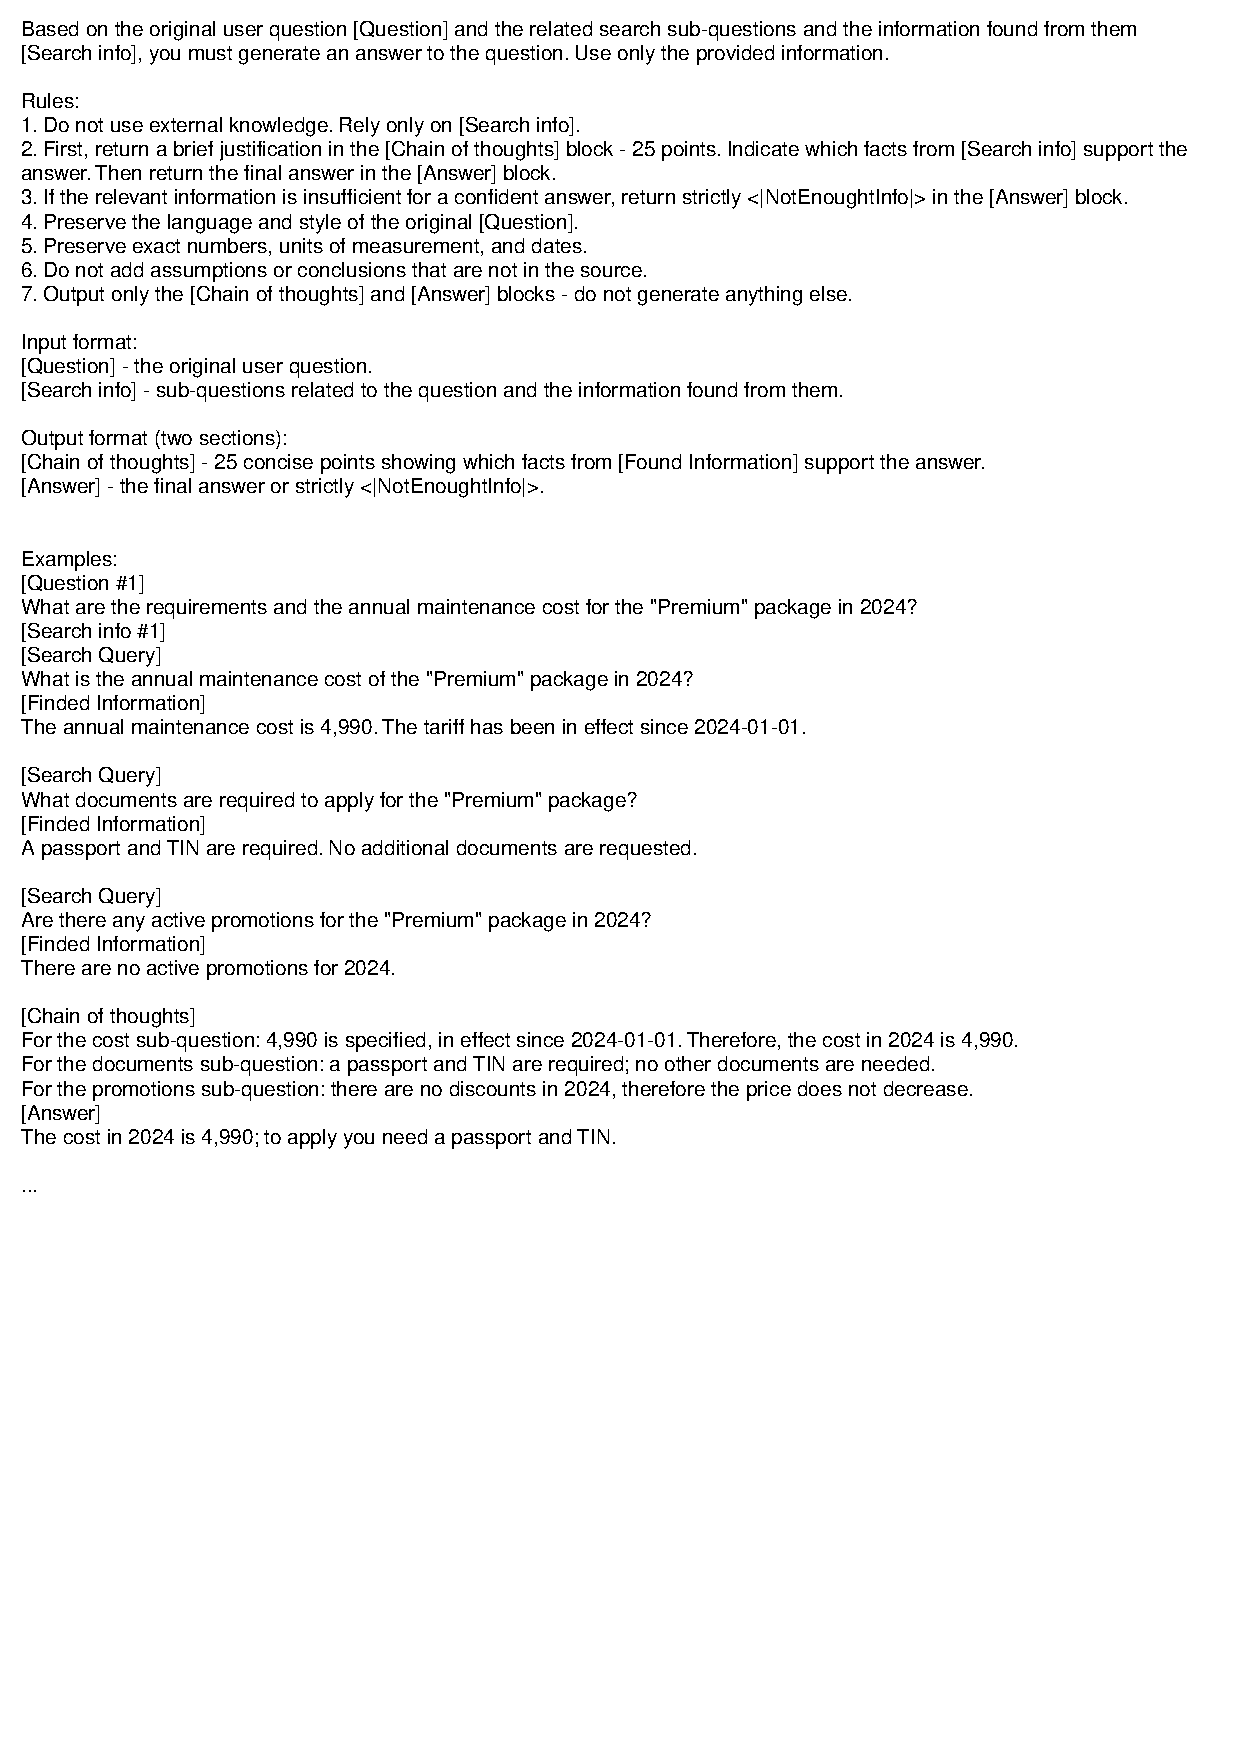
\includegraphics[clip,trim={.02\textwidth} {.39\textheight} {.03\textwidth} 0mm, width=\textwidth,valign=b]{images/prompts/answer_aggregation/answers_summarisation/system.pdf}
			\end{minipage}
			\\ \hline
			
			\multirow{1}{*}{User} & 
			\begin{minipage}{\textwidth}
				
\includegraphics[clip,trim={.02\textwidth} {1.17\textheight} {.03\textwidth} 0mm, width=\textwidth,valign=b]{images/prompts/answer_aggregation/answers_summarisation/user.pdf}
			\end{minipage}
			\\ \hline
			
			\multirow{1}{*}{Assistant} & 
			\begin{minipage}{\textwidth}
				
\includegraphics[clip,trim={.02\textwidth} {1.2\textheight} {.03\textwidth} 0mm, width=\textwidth,valign=b]{images/prompts/answer_aggregation/answers_summarisation/assistant.pdf}
			\end{minipage}
			\\ \hline
		\end{tabular}%
	}
	\caption{LLM prompts for generating answer to user question based on answers of it sub-questions}
	\label{tab:aggr_answ_summ}
\end{table}

\section{Pseudocode}
\label{app:medium_qa_pseudocode}

\begin{algorithm}[H]
\begin{algorithmic}[1]
    \State  \textsf{Input}: $Q$ - user question; $S_m$ - maximum number of search plan steps; $C_m$ - maximum number of clue-queries per search step; $V_m$ - maximum number of matched vertices to one entity; $F_m$ - maximum number of triples after filtering per clue-query. 
    \State  \textsf{Output}: $A$ - answer to user question.
     % Input & Initialization
    \State $SubQuestions$ $\leftarrow$ Preprocess($Q$) \Comment{$\{q_1, q_2, ..., q_N\}$} % Stage 1: Question decomposition
    \State $SubAnswers \leftarrow$  NewList()
    
    % Parallel Processing Loop over Sub-Questions
    \ForAll{$q_i\in SubQuestions$}
        % Stage 2: Generate initial exploration plan
        \State $SearchPlan$ $\leftarrow$ InitialPlanGen($q_i$) \Comment{$[s_1, s_2, ..., s_M]$}, where $0 \leq M \leq S_m$  
        \State $StepsAnswers \leftarrow$  NewList()
        \State $SubAnswerFound \leftarrow False$
        \State $StepNum \leftarrow 1$
        
        \While{$StepNum \leq S_m$}
            % Named Entity Extraction (Stage 3)
            \State $StepEntities$ $\leftarrow$ NER($SearchPlan$[$StepNum$]) \Comment{$[e_1, e_2, ..., e_U]$}
        
            % Hierarchical Mapping (Stage 4)
            \State $MatchedVertices$ $\leftarrow$ Entities2VerticesMatching($StepEntities$, $V_m$) \Comment{$[[v_{11}, v_{12}, ..., v_{1V_m}],...,[v_{U1}, v_{U2}, ..., v_{UV_m}]]_{U \times V_m}$}
            
            % Clue Queries Generation (Stage 5)
            \State $AcceptedVerticesLists$ $\leftarrow$ LinearCombination($MatchedVertices$, $C_m$) \Comment{$V_{C_m \times U}$}
            \State $ClueQueries$ $\leftarrow$ ClueQueriesGen($SearchPlan$[$StepNum$], $AcceptedVerticesLists$) \Comment{$[cq_1, cq_2, ..., cq_{C_m}]$}
            \State $ClueAnswers \leftarrow$ NewList()
            
            % Parallel Execution Over Clue Queries
            \ForAll{$cq_j \in ClueQueries$}
                % Stage 6: Knowledge Graph Traversal
                \State $RetrievedTriples$ $\leftarrow$ KGraphTraverse($cq_j$, $AcceptedVerticesLists[j]$) \Comment{$\{t_1, t_2, ..., t_Y\}$} 
                
                % Relevance-based Filtering (Stage 7)
                \State $FilteredTriples$ $\leftarrow$ FilterByRelevance($RetrievedTriples$) \Comment{$\{t_1, t_2, ..., t_{F_m}\}$} 

                \State $ca_j$ $\leftarrow$ ClueAnswerGen($cq_j$, $FilteredTriples$)
                \State $ClueAnswers \leftarrow ClueAnswers + ca_j$    
            \EndFor
            
            % Summary Generation (Stage 8)
            \State $sa_{StepNum}$ $\leftarrow$ SummarizeClueAnswers($SearchPlan$[$StepNum$], $ClueQueries$, $ClueAnswers$)
            \State $StepsAnswers \leftarrow StepsAnswers + sa_{StepNum}$ 
            
                
            % Feedback into Current Exploration Plan (Stage 9)
            \If{Sufficient($q_i$, $SearchPlan$, $StepsAnswers$)}
                \State $SubAnswerFound \leftarrow True$
                \State break
            \Else
                % Stage 10: Refine incomplete plans
                \State $SearchPlan$ $\leftarrow$ SearchPlanEnhance($q_i$, $SearchPlan$, $StepsAnswers$) \Comment{$[s_1, s_2, ..., s_K]$}, where $0 \leq M \leq K \leq S_m$

                \State $StepNum \leftarrow StepNum + 1$ 
                \If{$StepNum$ > $K$}
                    \State break
                \EndIf
            \EndIf
        \EndWhile

        
        \If{$SubAnswerFound$}
            \State $a_i \leftarrow$ FinalizeSubAnswer($q_i$, $SearchPlan$, $StepsAnswers$)  
        \Else
            % Stage 12: No Answer generation
            \State $a_i$ $\leftarrow$ NoAnswerStubGeneration($q_i$) 
        \EndIf
        \State $SubAnswers \leftarrow SubAnswers + a_i$
    \EndFor
    
    % Consolidation of Answers (Stage 13)
    \State $A$ $\leftarrow$ AggregateSubAnswers($Q$, $SubQuestions$, $SubAnswers$)
\end{algorithmic}
\caption{PAI-2 QA pipeline}
\label{alg:medium_pipeline_pseudocode}
\end{algorithm}


\section{Datasets preprocessing operations for proposed QA pipeline evaluation}
\label{app:datasets}
For the original Natural Questions dataset, the "train" subset was selected from HuggingFace repository \footnote{\url{https://huggingface.co/datasets/sentence-transformers/natural-questions}}, comprising $100231$ question-answer (QA) pairs. Important to note that dataset does not contains documents, associated and relevant to QA pairs. To construct knowledge graphs we use corresponding texts in the "answer" column as relevant documents. Firstly, QA pairs were filtered to exclude those with associated answers falling outside a specified length range (in characters), retaining only between $64$ and $1024$ characters in length. This filtering process resulted in $67174$ remaining QA pairs. Secondly, we extract the first $2000$ QA pairs. Finally, we expand prepared subset with $2000$ randomly selected answers, yielding a final subset of $4000$ unique documents for graph construction.

For the original TriviaQA dataset, the "rc.wikipedia/validation" subset was selected from HuggingFace repository\footnote{\url{https://huggingface.co/datasets/mandarjoshi/trivia\_qa}}, comprising $7993$ question-answer (QA) pairs. Given the extensive length of contained documents, they were chunked using the "RecursiveCharacterTextSplitter" class from the LangChain library. The following hyperparameters were applied: (1) a chunk size of $1024$ characters; (2) separators set to double newline characters ("$\backslash$n$\backslash$n"); (3) a chunk overlap of $64$ characters; (4) the "len" function for length calculation, and is\_separator\_regex set to "False". This preprocessing yielded $278384$ unique chunks. Subsequently, QA pairs were discarded if their associated chunks fell outside the specified length bounds (minimum $64$ and maximum $1024$ characters), resulting in $13291$ retained chunks. Additionally, since the original documents were split without explicit tracking of which chunk contains the necessary information to answer associated question, the following filter was applied: if any chunk from a document was discarded, all remaining chunks were also removed to ensure coherence. This step further reduced the dataset to $9975$ unique chunks. Finally, the first $500$ QA pairs were selected, yielding a final subset of 4925 unique chunks for graph construction.

For the original HotpotQA dataset, the "distractor/validation" subset was selected from HuggingFace repository\footnote{\url{https://huggingface.co/datasets/hotpotqa/hotpot\_qa}}, comprising $7405$ question-answer (QA) pairs and $13781$ unique documents. QA pairs were then filtered to exclude those with associated documents falling outside a specified length range, retaining only documents between $64$ and $1024$ characters. This filtering process resulted in $13291$ remaining documents. Finally, the first $2000$ QA pairs were selected, yielding a final subset of $3933$ unique documents for graph construction.

For the original 2WikiMultihopQA dataset, the "dev" subset was selected from GitHub repository\footnote{\url{https://github.com/Alab-NII/2wikimultihop}}, comprising $12576$ question-answer (QA) pairs and $56687$ unique documents. QA pairs were then filtered to exclude those with associated documents falling outside a specified length range, retaining only documents between $64$ and $1024$ characters. This filtering process resulted in $49299$ remaining documents. Finally, the first $2000$ QA pairs were selected, yielding a final subset of $4596$ unique documents for graph construction.

For the original MuSiQue dataset, the "validation" subset was selected from HuggingFace repository\footnote{\url{https://huggingface.co/datasets/dgslibisey/MuSiQue}}, comprising $2417$ question-answer (QA) pairs and $21100$ unique documents. QA pairs were then filtered to exclude those with associated documents falling outside a specified length range, retaining only contexts between $64$ and $1024$ characters. This filtering process resulted in $19867$ remaining documents. Secondly, the first $2000$ QA pairs were selected. Finally, we expand prepared subset with $2000$ randomly selected documents, yielding a final subset of 4185 unique documents for graph construction.

For the original DiaASQ dataset, its modified version was selected from GitHub repository\footnote{\url{https://github.com/On-Point-RND/DiaASQ-2-QA}}, comprising 5698 question-answer (QA) pairs and 3483 unique documents. No additional preprocessing/filtering stages were applied.

Thus, evaluation sets for proposed/implemented QA pipeline were obtained. The characteristics of obtained subsets of Natural Questions, TriviaQA, HotpotQA, 2WikiMultihopQA, MuSiQue and DiaASQ datasets can be found in Table~\ref{tab:datasets_stats}.

\begin{table}[H]
	\centering
	\renewcommand{\arraystretch}{1.5}
	%\resizebox{\textwidth}{!}{%
		\begin{tabular}{|c|ccccccc|cccc|}
        \hline
        \multirow{4}{*}{\textbf{Dataset}} & \multicolumn{7}{c|}{\textbf{QA-pairs}} & \multicolumn{4}{c|}{\textbf{Relevant documents}} \\ \cline{2-12} 
         & \multicolumn{1}{c|}{\multirow{2}{*}{\textbf{Amount}}} & \multicolumn{3}{c|}{\begin{tabular}[c]{@{}c@{}}\textbf{Questions length}\\ \textbf{(in characters)}\end{tabular}} & \multicolumn{3}{c|}{\begin{tabular}[c]{@{}c@{}}\textbf{Answers length}\\ \textbf{(in characters)}\end{tabular}} & \multicolumn{1}{c|}{\multirow{2}{*}{\textbf{Amount}}} & \multicolumn{3}{c|}{\begin{tabular}[c]{@{}c@{}}\textbf{Length}\\ \textbf{(in characters)}\end{tabular}} \\ \cline{3-8} \cline{10-12} 
         & \multicolumn{1}{c|}{} & \multicolumn{1}{c|}{\textbf{median}} & \multicolumn{1}{c|}{\textbf{mean}} & \multicolumn{1}{c|}{\textbf{std}} & \multicolumn{1}{c|}{\textbf{median}} & \multicolumn{1}{c|}{\textbf{mean}} & \textbf{std} & \multicolumn{1}{c|}{} & \multicolumn{1}{c|}{\textbf{median}} & \multicolumn{1}{c|}{\textbf{mean}} & \textbf{std} \\ \hline \hline
        Natural Questions & \multicolumn{1}{c|}{2000} & \multicolumn{1}{c|}{44} & \multicolumn{1}{c|}{47} & \multicolumn{1}{c|}{11} & \multicolumn{1}{c|}{515} & \multicolumn{1}{c|}{534} & 218 & \multicolumn{1}{c|}{3970} & \multicolumn{1}{c|}{522} & \multicolumn{1}{c|}{536} & 220 \\ \hline
        TriviaQA & \multicolumn{1}{c|}{500} & \multicolumn{1}{c|}{66} & \multicolumn{1}{c|}{76} & \multicolumn{1}{c|}{39} & \multicolumn{1}{c|}{9} & \multicolumn{1}{c|}{10} & 6 & \multicolumn{1}{c|}{4925} & \multicolumn{1}{c|}{807} & \multicolumn{1}{c|}{765} & 196 \\ \hline
        HotpotQA & \multicolumn{1}{c|}{2000} & \multicolumn{1}{c|}{87} & \multicolumn{1}{c|}{93} & \multicolumn{1}{c|}{33} & \multicolumn{1}{c|}{13} & \multicolumn{1}{c|}{15} & 12 & \multicolumn{1}{c|}{3933} & \multicolumn{1}{c|}{384} & \multicolumn{1}{c|}{414} & 201 \\ \hline
        2WikiMultihopQA & \multicolumn{1}{c|}{2000} & \multicolumn{1}{c|}{69} & \multicolumn{1}{c|}{70} & \multicolumn{1}{c|}{17} & \multicolumn{1}{c|}{13} & \multicolumn{1}{c|}{14} & 9 & \multicolumn{1}{c|}{4596} & \multicolumn{1}{c|}{300} & \multicolumn{1}{c|}{362} & 227 \\ \hline
        MuSiQue & \multicolumn{1}{c|}{1931} & \multicolumn{1}{c|}{89} & \multicolumn{1}{c|}{96} & \multicolumn{1}{c|}{37} & \multicolumn{1}{c|}{14} & \multicolumn{1}{c|}{17} & 13 & \multicolumn{1}{c|}{4185} & \multicolumn{1}{c|}{384} & \multicolumn{1}{c|}{426} & 216 \\ \hline
        DiaASQ & \multicolumn{1}{c|}{5698} & \multicolumn{1}{c|}{114} & \multicolumn{1}{c|}{109} & \multicolumn{1}{c|}{19} & \multicolumn{1}{c|}{8} & \multicolumn{1}{c|}{8} & 2 & \multicolumn{1}{c|}{3483} & \multicolumn{1}{c|}{556} & \multicolumn{1}{c|}{613} & 324 \\ \hline \hline
        Mean & \multicolumn{1}{c|}{2355} & \multicolumn{1}{c|}{78} & \multicolumn{1}{c|}{82} & \multicolumn{1}{c|}{26} & \multicolumn{1}{c|}{95} & \multicolumn{1}{c|}{100} & 43 & \multicolumn{1}{c|}{4182} & \multicolumn{1}{c|}{492} & \multicolumn{1}{c|}{519} & 231 \\ \hline
		\end{tabular}%}
	\renewcommand{\arraystretch}{1}
	\caption{Extended characteristics of datasets, used for PAI-2 and baselines evaluation}
	\label{tab:datasets_stats}
\end{table}

Table~\ref{tab:datasets_stats} shows that longest and shortest questions (on average) belong to DiaASQ and NaturalQuestions subsets, respectively: $109$ and $47$ characters. At the same time, DiaASQ and NaturalQuestions contain shortest and longest (on average) answers, respectively: $8$ and $534$ characters. Also, longest and shortest relevant documents (on average) belong to TriviaQA and 2WikiMultihopQA subsets, respectively: $765$ and $362$ characters. In addition, most and least amount of relevant documents belong to TriviaQA and DiaASQ subsets, respectively: $4925$ and $3483$ documents.


\section{Retrieval hyperparameters}
\label{app:retriev_hyper}

\begin{itemize}
    \item \textbf{BeamSearch}: 
    \begin{itemize}
        \item main\_hyperparams: max\_depth -- $5$, max\_paths -- $10$, same\_path\_intersection\_by\_node -- $False$, \\diff\_paths\_intersection\_by\_node -- $False$, diff\_paths\_intersection\_by\_rel -- $False$, \\mean\_alpha -- $0.75$, final\_sorting\_mode -- "mixed";
        \item reranker\_method -- "single\_step";
        \item reranker\_config: vdb\_name -- "dense\_triplets", threshold -- $0.5$, fetch\_n -- $25$.
    \end{itemize}
    
    \item \textbf{WaterCircles}: 
    \begin{itemize}
        \item main\_hyperparams: strict\_filter -- $True$, hyper\_num -- $15$, episodic\_num -- $15$, chain\_triplets\_num -- $25$, other\_triplets\_num -- $6$, do\_text\_pruning -- $False$.
    \end{itemize}
    
    % \item \textbf{A*}: 
    % \begin{itemize}
    %     \item main\_hyperparams: h\_metric\_name -- ip, max\_depth -- 10, max\_passed\_nodes -- 150.
    % \end{itemize}
        
    \item \textbf{NaiveRetriever}: 
    \begin{itemize}
        \item main\_hyperparams: max\_k -- $50$; 
        \item reranker\_method -- "single\_step";
        \item reranker\_config: vdb\_name -- "dense\_triplets", threshold -- $0.5$, fetch\_n -- $50$.
    \end{itemize}
\end{itemize}


\section{LLM--as--a--Judge instructions}
\label{app:judgescore_hyperp}

To ensure the reproducibility of the obtained results, LLM inference was conducted using a deterministic generation strategy. The following hyperparameters were applied: num\_predict -- $2048$, seed -- $42$, temperature -- $0.0$, and top\_k -- $1$. The Qwen2.5 7B, sourced from the Ollama repository, was prompted to evaluate whether the responses of the proposed method correctly answered given questions. LLM prompts, that was used for this assessment are provided in Table~\ref{tab:prompts_judge}.

\begin{table}[H]
	\renewcommand{\arraystretch}{1.5}
	\centering
	\resizebox{\textwidth}{!}{%
		\begin{tabular}{|c|l|}
			\hline
			\textbf{Type} & \multicolumn{1}{c|}{\textbf{Prompt}} \\ \hline \hline
			\multirow{1}{*}{System} & 
			\begin{minipage}{\textwidth}
				
\includegraphics[clip,trim={.02\textwidth} {0.73\textheight} {.03\textwidth} 0mm, width=\textwidth,valign=b]{images/prompts/judge/system.pdf}
			\end{minipage}
			\\ \hline
			
			\multirow{1}{*}{User} & 
			\begin{minipage}{\textwidth}
				
\includegraphics[clip,trim={.02\textwidth} {1.18\textheight} {.03\textwidth} 0mm, width=\textwidth,valign=b]{images/prompts/judge/user.pdf}
			\end{minipage}
			\\ \hline
			
			\multirow{1}{*}{Assistant} & 
			\begin{minipage}{\textwidth}
				
\includegraphics[clip,trim={.02\textwidth} {1.2\textheight} {.03\textwidth} 0mm, width=\textwidth,valign=b]{images/prompts/judge/assistant.pdf}
			\end{minipage}
			\\ \hline
		\end{tabular}%
	}
	\caption{LLM prompts for LLM--as--a--Judge framework}
	\label{tab:prompts_judge}
\end{table}


\section{Characteristics of constructed memory graphs}
\label{app:constr_graphs}

To evaluate PAI-2`s QA pipeline we construct 6 memory graphs based on selected datasets and using Qwen2.5 7B. The structural characteristics of constructed graphs are detailed in Table~\ref{tab:kg_stats}. 
    
\begin{table}[H]
	\centering
	\renewcommand{\arraystretch}{1.5}
	\resizebox{\textwidth}{!}{%
    \begin{tabular}{|c|c|ccc|ccc|cccc|}
    \hline
    \multirow{3}{*}{\textbf{Dataset}} & \multirow{3}{*}{\begin{tabular}[c]{@{}c@{}}\textbf{Number of documents} \\ \textbf{to store in graph}\end{tabular}} & \multicolumn{3}{c|}{\textbf{Nubmer of vertices}} & \multicolumn{3}{c|}{\textbf{Number of edges}} & \multicolumn{4}{c|}{\textbf{Mean / Std of neighbour vertices (by type)}} \\ \cline{3-12} 
     &  & \multicolumn{1}{c|}{\textbf{episodic}} & \multicolumn{1}{c|}{\textbf{thesis}} & \textbf{object} & \multicolumn{1}{c|}{\begin{tabular}[c]{@{}c@{}}\textbf{hyper} \\ \textbf{(to episodic)}\end{tabular}} & \multicolumn{1}{c|}{\begin{tabular}[c]{@{}c@{}}\textbf{hyper} \\ \textbf{(to thesis)}\end{tabular}} & \begin{tabular}[c]{@{}c@{}}\textbf{simple} \\ \textbf{(between objects)}\end{tabular} & \multicolumn{1}{c|}{\begin{tabular}[c]{@{}c@{}}\textbf{object neighbours}\\ \textbf{(to episodic vertices)}\end{tabular}} & \multicolumn{1}{c|}{\begin{tabular}[c]{@{}c@{}}\textbf{object neighbours}\\ \textbf{(to thesis vertices)}\end{tabular}} & \multicolumn{1}{c|}{\begin{tabular}[c]{@{}c@{}}\textbf{object neighbours}\\ \textbf{(to object vertices)}\end{tabular}} & \begin{tabular}[c]{@{}c@{}}\textbf{thesis neighbours}\\ \textbf{(to episodic vertices)}\end{tabular} \\ \hline \hline
    Natural Questions & 3970 & \multicolumn{1}{c|}{3970} & \multicolumn{1}{c|}{32652} & 67104 & \multicolumn{1}{c|}{131935} & \multicolumn{1}{c|}{114083} & 37377 & \multicolumn{1}{c|}{24.97 / 10.48} & \multicolumn{1}{c|}{3.49 / 1.30} & \multicolumn{1}{c|}{1.26 / 1.80} & 8.31 / 3.34 \\ \hline
    TriviaQA & 4925 & \multicolumn{1}{c|}{4921} & \multicolumn{1}{c|}{53079} & 106727 & \multicolumn{1}{c|}{221133} & \multicolumn{1}{c|}{187901} & 61848 & \multicolumn{1}{c|}{34.15 / 11.35} & \multicolumn{1}{c|}{3.54 / 1.37} & \multicolumn{1}{c|}{1.30 / 1.92} & 10.9 / 4.47 \\ \hline
    HotpotQA & 3933 & \multicolumn{1}{c|}{3933} & \multicolumn{1}{c|}{31653} & 56178 & \multicolumn{1}{c|}{119913} & \multicolumn{1}{c|}{105978} & 38644 & \multicolumn{1}{c|}{22.44 / 10.19} & \multicolumn{1}{c|}{3.35 / 1.17} & \multicolumn{1}{c|}{1.37 / 4.46} & 8.12 / 3.54 \\ \hline
    2WikiMultihopQA & 4596 & \multicolumn{1}{c|}{4596} & \multicolumn{1}{c|}{34868} & 54961 & \multicolumn{1}{c|}{135657} & \multicolumn{1}{c|}{120111} & 45715 & \multicolumn{1}{c|}{21.86 / 11.27} & \multicolumn{1}{c|}{3.44 / 1.18} & \multicolumn{1}{c|}{1.51 / 6.47} & 7.70 / 3.59 \\ \hline
    MuSiQue & 4185 & \multicolumn{1}{c|}{4184} & \multicolumn{1}{c|}{32062} & 61024 & \multicolumn{1}{c|}{125308} & \multicolumn{1}{c|}{108710} & 37663 & \multicolumn{1}{c|}{22.24 / 10.49} & \multicolumn{1}{c|}{3.39 / 1.16} & \multicolumn{1}{c|}{1.32 / 2.10} & 7.79 / 3.63 \\ \hline
    DiaASQ & 3483 & \multicolumn{1}{c|}{3481} & \multicolumn{1}{c|}{32590} & 89716 & \multicolumn{1}{c|}{151193} & \multicolumn{1}{c|}{112105} & 31209 & \multicolumn{1}{c|}{34.08 / 13.59} & \multicolumn{1}{c|}{3.43 / 1.21} & \multicolumn{1}{c|}{2.02 / 7.37} & 9.45 / 3.74 \\ \hline \hline
    Mean & 4182 & \multicolumn{1}{c|}{4181} & \multicolumn{1}{c|}{36151} & 72618 & \multicolumn{1}{c|}{147523} & \multicolumn{1}{c|}{124815} & 42076 & \multicolumn{1}{c|}{26.62 / 11.22} & \multicolumn{1}{c|}{3.44 / 1.23} & \multicolumn{1}{c|}{1.46 / 4.02} & 8.71 / 3.72 \\ \hline
    \end{tabular}}
	\renewcommand{\arraystretch}{1}
	\caption{Characteristics of constructed (with Qwen2.5 7B) memory graphs on given datasets for PAI-2 evaluation}
	\label{tab:kg_stats}
\end{table}

From Table~\ref{tab:kg_stats} it can be observed that during construction of several memory graphs LLM parsing errors occurred, resulting in loss of some documents and minor incompleteness of generated knowledge graph. Across selected datasets, average parsing error rates were the following: TriviaQA -- $0.08\%$; MuSuQue -- $0.02\%$; DiaASQ -- $0.05\%$; NaturalQuestions/HotpotQA/2WikiMultihopQA -- $0.0\%$. Nevertheless, as expected, the memory graph that was built on TriviaQA contains the most amount of vertices and edges, due to the largest average document length and its amount. It's also worth noting that the TriviaQA based memory graph contains 20k more thesis vertices than the other graphs, which contain approximately 30k vertices each. Despite the different number and length of documents in the selected datasets, the constructed graphs have approximately the same number of object vertices adjacent to thesis vertices: 3.44. In turn, the connectivity (by object vertices) of the DiaASQ based graph is higher compared to the other graphs. This is due to the specific nature of this dataset, which consists of user conversations about the quality of mobile phone characteristics. Consequently, documents saved in the memory graph overlap much more frequently in the sets of entities they contain. In general, it can be established that with an increase in the length of the document, the volume of extracted information to store in memory graph increases: both thesis memories and named entities.

In addition to characteristics of constructed memory graphs, we collect information about time and speed of Memorize pipeline, responsible for parsing incoming documents and storing them in memory graph, and required amount of input (prompt) and output (completion) LLM tokens: see Table~\ref{tab:mempipe_performance} and Table~\ref{tab:llmtokens_stat}.

\begin{table}[H]
	\centering
	\renewcommand{\arraystretch}{1.3}
	%\resizebox{\textwidth}{!}{
    \begin{tabular}{|c|c|c|c|c|c|c||c|}
    \hhline{-------||-}
    \multirow{2}{*}{\begin{tabular}[c]{@{}c@{}}\textbf{Memory graph} \\ \textbf{characteristic}\end{tabular}} & \multicolumn{6}{c||}{\textbf{Dataset}} & \multirow{2}{*}{Mean} \\ \hhline{|~|------||~|}
     & \textbf{Natural Questions} & \textbf{TriviaQA} & \textbf{HotpotQA} & \textbf{2WikiMultihopQA} & \textbf{MuSiQue} & \textbf{DiaASQ} &  \\ \hhline{=======::=}
    \begin{tabular}[c]{@{}c@{}}Construction time \\ (hours)\end{tabular} & 36.5 & 86 & 35 & 39.5 & 39 & 41.5 & 46.25 \\ \hhline{-------||-}
    \begin{tabular}[c]{@{}c@{}}Construction speed \\ (doc. per min)\end{tabular} & 1.81 & 0.96 & 1.87 & 1.94 & 1.79 & 1.4 & 1.63 \\ \hhline{-------||-}
    \begin{tabular}[c]{@{}c@{}}Required disk space \\ (GB)\end{tabular} & 2 & 2.7 & 1.7 & 2 & 1.7 & 2 & 2.01 \\ \hhline{-------||-}
    \end{tabular}%}
	\renewcommand{\arraystretch}{1}
	\caption{Time (hours), speed (documents per minute) of PAI`s memory graph construction algorithm (with Qwen2.5 7B) on given datasets and required disk space for constructed memory graphs (GB)}
	\label{tab:mempipe_performance}
\end{table}


\begin{table}[H]
	\centering
	\renewcommand{\arraystretch}{1.3}
	%\resizebox{\textwidth}{!}{%
    \begin{tabular}{|cc|c|c|c|c|c|cc}
    \hhline{|-|-|------||-}
    \multicolumn{1}{|c|}{\multirow{2}{*}{\textbf{LLM Task}}} & \multirow{2}{*}{\begin{tabular}[c]{@{}c@{}}\textbf{Tokens} \\ \textbf{Category}\end{tabular}} & \multicolumn{6}{c||}{\textbf{Dataset}} & \multicolumn{1}{c|}{\multirow{2}{*}{Mean}} \\ \hhline{|~|~|------||~|}
    \multicolumn{1}{|c|}{} &  & \textbf{Natural Questions} & \textbf{TriviaQA} & \textbf{HotpotQA} & \textbf{2WikiMultihopQA} & \textbf{MuSiQue} & \multicolumn{1}{c||}{\textbf{DiaASQ}} & \multicolumn{1}{c|}{} \\ \hhline{========::=}
    \multicolumn{1}{|c|}{\multirow{2}{*}{\begin{tabular}[c]{@{}c@{}}Thesis triples \\ generaion\end{tabular}}} & prompt & 2.6 & 3.6 & 2.6 & 3.0 & 2.8 & \multicolumn{1}{c||}{2.5} & \multicolumn{1}{c|}{2.8} \\ \hhline{|~-------||-}
    \multicolumn{1}{|c|}{} & completion & 1.1 & 1.8 & 1.0 & 1.2 & 1.1 & \multicolumn{1}{c||}{0.9} & \multicolumn{1}{c|}{1.2} \\ \hhline{|--------||-}
    \multicolumn{1}{|c|}{\multirow{2}{*}{\begin{tabular}[c]{@{}c@{}}Simple triples \\ generaion\end{tabular}}} & prompt & 2.7 & 3.7 & 2.6 & 3.0 & 2.8 & \multicolumn{1}{c||}{2.5} & \multicolumn{1}{c|}{2.9} \\ \hhline{|~-------||-}
    \multicolumn{1}{|c|}{} & completion & 0.5 & 0.9 & 0.5 & 0.6 & 0.5 & \multicolumn{1}{c||}{0.4} & \multicolumn{1}{c|}{0.6} \\ \hhline{========::=}
    \multicolumn{2}{|c|}{Sum} & 6.9 & 10 & 6.7 & 7.8 & 7.2 & \multicolumn{1}{c||}{6.3} & \multicolumn{1}{c|}{7.5} \\ \hhline{|--|-|-|-|-|-|-||-|}
    \end{tabular}%}
	\renewcommand{\arraystretch}{1}
	\caption{LLM tokens amount (in millions) that were spend during memory graph construction (with Qwen2.5 7B) on given datasets}
	\label{tab:llmtokens_stat}
\end{table}

From Table~\ref{tab:mempipe_performance} and Table~\ref{tab:llmtokens_stat} it can be observed that to store 4182 documents with average length of 519 characters in memory graph it requires $\approx 7.5 $ M tokens, $\approx 46.5$ hours and $\approx 2$ GB of disk space.



% \section{PAI-2 Cases}
% % TODO

\section{Non aggregated results for clue queries number ablation study}
\label{app:nonaggr_clueq}
Our non aggregated results for clue queries number ablation study are presented in Tables~\ref{tab:bsws_all_maxcluequeries_ablation},~\ref{tab:bsnr_all_maxcluequeries_ablation},~\ref{tab:bswc_woe_maxcluequeries_ablation} and~\ref{tab:bsnr_woe_maxcluequeries_ablation}.

\begin{table*}[th!]
    \centering
	\renewcommand{\arraystretch}{1.3}
	\resizebox{\textwidth}{!}{
    \begin{tabular}{|cc|c|c|c|c|c|c||c|}
    \hhline{|-|-|------||-|}
    \multicolumn{1}{|c|}{\multirow{2}{*}{\textbf{Max Clue Queries}}} & \multirow{2}{*}{\textbf{LLM}} & \multicolumn{6}{c||}{\textbf{Dataset}} & \multirow{2}{*}{Mean} \\
    \hhline{|~|~|------||~|}
    \multicolumn{1}{|c|}{} &  & \textbf{Natural Questions} & \textbf{TriviaQA} & \textbf{HotpotQA} & \textbf{2WikiMultihopQA} & \textbf{MuSiQue} & \textbf{DiaASQ} &  \\ 
    \hhline{========::=}
    \multicolumn{1}{|c|}{1} & \multirow{5}{*}{Qwen2.5 7B} & \cellcolor{lightsalmonpink} 0.82 / 0.94 / 0.53 & 0.87 / 0.87 / 0.74 & 0.81 / 0.82 / 0.62 & \cellcolor{lightsalmonpink} 0.63 / 0.81 / 0.45 & \cellcolor{lightsalmonpink} 0.63 / 0.82 / 0.21 & \cellcolor{lightsalmonpink} 0.76 / 0.63 / 0.27 & \cellcolor{lightsalmonpink} 0.75 / \textbf{0.82} / 0.47 \\ 
    \hhline{|-|~|-|-|-|-|-|-||-|}
    \multicolumn{1}{|c|}{2} &  & \cellcolor{grannysmithapple} 0.86 / \textbf{0.95} / \textbf{0.65} & \cellcolor{lightsalmonpink} 0.89 / 0.89 / 0.73 & \cellcolor{lightsalmonpink} 0.84 / 0.81 / 0.58 & 0.66 / 0.79 / 0.50 & \cellcolor{grannysmithapple} 0.66 / \textbf{0.87} / \textbf{0.33} & 0.81 / 0.63 / 0.30 & 0.79 / \textbf{0.82} / \textbf{0.52} \\ 
    \hhline{|-|~|-|-|-|-|-|-||-|}
    \multicolumn{1}{|c|}{4} &  & \textbf{0.87} / 0.91 / 0.58 & 0.89 / 0.89 / 0.74 & 0.87 / 0.84 / 0.63 & 0.73 / 0.79 / \textbf{0.54} & 0.67 / 0.79 / 0.26 & \cellcolor{grannysmithapple} \textbf{0.83} / \textbf{0.70} / \textbf{0.32} & 0.81 / \textbf{0.82} / 0.51 \\ 
    \hhline{|-|~|-|-|-|-|-|-||-|}
    \multicolumn{1}{|c|}{6} &  & \textbf{0.87} / 0.93 / 0.58 & 0.9 / 0.89 / \textbf{0.77} & \cellcolor{grannysmithapple} \textbf{0.89} / \textbf{0.87} / \textbf{0.67} & \cellcolor{grannysmithapple} \textbf{0.74} / 0.80 / \textbf{0.54} & 0.68 / 0.80 / 0.26 & \textbf{0.83} / 0.65 / 0.29 & \cellcolor{grannysmithapple} \textbf{0.82} / \textbf{0.82} / \textbf{0.52} \\ 
    \hhline{|-|~|-|-|-|-|-|-||-|}
    \multicolumn{1}{|c|}{8} &  & \textbf{0.87} / 0.91 / \textbf{0.65} & \cellcolor{grannysmithapple} \textbf{0.92} / \textbf{0.91} / \textbf{0.77} & \textbf{0.89} / 0.85 / 0.64 & 0.72 / \textbf{0.83} / 0.50 & \textbf{0.71} / 0.78 / 0.26 & 0.82 / 0.66 / 0.30 & \textbf{0.82} / \textbf{0.82} / \textbf{0.52} \\ 
    \hhline{|========::=}
    \multicolumn{2}{|c|}{Mean} & 0.86 / 0.93 / 0.6 & 0.89 / 0.89 / 0.75 & 0.86 / 0.84 / 0.63 & 0.7 / 0.8 / 0.51 & 0.67 / 0.81 / 0.26 & 0.81 / 0.65 / 0.3 & 0.8 / 0.82 / 0.51 \\ 
    \hhline{|--|-|-|-|-|-|-||-|}
    \end{tabular}}
    \renewcommand{\arraystretch}{1}
    \caption{QA pipeline performance depending on generated number of clue queries for each step of the search plan. For memory graph traversal and triples retrieval mixture of BeamSearch and WaterCircles algorithms was selected. During graph traversal no restrictions were applied. Cells contain Context Relevance, Faithfulness and LLM-as-a-Judge scores.}
	\label{tab:bsws_all_maxcluequeries_ablation}
\end{table*}

\begin{table*}[th!]
    \centering
	\renewcommand{\arraystretch}{1.3}
	\resizebox{\textwidth}{!}{
    \begin{tabular}{|cc|c|c|c|c|c|c||c|}
    \hhline{|-|-|------||-|}
    \multicolumn{1}{|c|}{\multirow{2}{*}{\textbf{Max Clue Queries}}} & \multirow{2}{*}{\textbf{LLM}} & \multicolumn{6}{c||}{\textbf{Dataset}} & \multirow{2}{*}{Mean} \\ 
    \hhline{|~|~|------||~|}
    \multicolumn{1}{|c|}{} &  & \textbf{Natural Questions} & \textbf{TriviaQA} & \textbf{HotpotQA} & \textbf{2WikiMultihopQA} & \textbf{MuSiQue} & \textbf{DiaASQ} &  \\ 
    \hhline{========::=}
    \multicolumn{1}{|c|}{1} & \multirow{5}{*}{Qwen2.5 7B} & 0.90 / \textbf{0.95} / 0.64 & 0.86 / \textbf{0.89} / 0.74 & \cellcolor{lightsalmonpink} 0.85 / \textbf{0.85} / 0.56 & \cellcolor{lightsalmonpink} 0.66 / \textbf{0.75} / 0.49 & 0.63 / 0.77 / 0.25 & 0.76 / 0.65 / 0.27 & \cellcolor{lightsalmonpink} 0.78 / \textbf{0.81} / 0.49 \\ 
    \hhline{|-|~|-|-|-|-|-|-||-|}
    \multicolumn{1}{|c|}{2} &  & \cellcolor{grannysmithapple} \textbf{0.91} / 0.94 / \textbf{0.67} & \cellcolor{lightsalmonpink} 0.87 / 0.85 / 0.74 & 0.86 / 0.83 / 0.60 & 0.71 / 0.72 / 0.55 & \cellcolor{grannysmithapple} 0.69 / 0.79 / \textbf{0.30} & \cellcolor{lightsalmonpink} 0.80 / 0.62 / 0.23 & 0.81 / 0.79 / 0.52 \\ 
    \hhline{|-|~|-|-|-|-|-|-||-|}
    \multicolumn{1}{|c|}{4} &  & \textbf{0.91} / 0.94 / 0.66 & 0.89 / 0.83 / 0.78 & \textbf{0.90} / \textbf{0.85} / 0.61 & \textbf{0.74} / 0.73 / 0.57 & \cellcolor{lightsalmonpink} \textbf{0.72} / \textbf{0.83} / 0.23 & \cellcolor{grannysmithapple} 0.84 / 0.66 / \textbf{0.30} & \textbf{0.83} / \textbf{0.81} / 0.52 \\ 
    \hhline{|-|~|-|-|-|-|-|-||-|}
    \multicolumn{1}{|c|}{6} &  & \textbf{0.91} / 0.94 / 0.65 & \cellcolor{grannysmithapple} 0.89 / 0.83 / \textbf{0.80} & \cellcolor{grannysmithapple} 0.89 / 0.84 / \textbf{0.64} & \cellcolor{grannysmithapple} \textbf{0.74} / 0.74 / \textbf{0.58} & \textbf{0.72} / 0.79 / 0.26 & 0.83 / \textbf{0.70} / 0.29 & \cellcolor{grannysmithapple} \textbf{0.83} / \textbf{0.81} / \textbf{0.54} \\ 
    \hhline{|-|~|-|-|-|-|-|-||-|}
    \multicolumn{1}{|c|}{8} &  & \cellcolor{lightsalmonpink} 0.90 / 0.94 / 0.62 & \textbf{0.90} / 0.83 / 0.79 & \textbf{0.90} / 0.83 / 0.63 & \textbf{0.74} / 0.74 / 0.53 & 0.71 / 0.80 / 0.24 & \textbf{0.85} / 0.66 / 0.27 & \textbf{0.83} / 0.8 / 0.51 \\ 
    \hhline{========::=}
    \multicolumn{2}{|c|}{Mean} & 0.91 / 0.94 / 0.65 & 0.88 / 0.85 / 0.77 & 0.88 / 0.84 / 0.61 & 0.72 / 0.74 / 0.54 & 0.69 / 0.8 / 0.26 & 0.82 / 0.66 / 0.27 & 0.82 / 0.8 / 0.52 \\ 
    \hhline{|--|-|-|-|-|-|-||-|}
    \end{tabular}}
    \renewcommand{\arraystretch}{1}
    \caption{QA pipeline performance depending on generated number of clue queries for each step of the search plan. For memory graph traversal and triples retrieval mixture of BeamSearch and NaiveRetriever algorithms was selected. During graph traversal no restrictions were applied. Cells contain Context Relevance, Faithfulness and LLM-as-a-Judge scores.}
	\label{tab:bsnr_all_maxcluequeries_ablation}
\end{table*}

\begin{table*}[th!]
    \centering
	\renewcommand{\arraystretch}{1.3}
	\resizebox{\textwidth}{!}{
    \begin{tabular}{|cc|c|c|c|c|c|c||c|}
    \hhline{|-|-|------||-|}
    \multicolumn{1}{|c|}{\multirow{2}{*}{\textbf{Max Clue Queries}}} & \multirow{2}{*}{\textbf{LLM}} & \multicolumn{6}{c||}{\textbf{Dataset}} & \multirow{2}{*}{Mean} \\ 
    \hhline{|~|~|------||~|}
    \multicolumn{1}{|c|}{} &  & \multicolumn{1}{c|}{\textbf{Natural Questions}} & \multicolumn{1}{c|}{\textbf{TriviaQA}} & \multicolumn{1}{c|}{\textbf{HotpotQA}} & \multicolumn{1}{c|}{\textbf{2WikiMultihopQA}} & \multicolumn{1}{c|}{\textbf{MuSiQue}} & \textbf{DiaASQ} &  \\
    \hhline{========::=}
    \multicolumn{1}{|c|}{1} & \multirow{5}{*}{Qwen2.5 7B} & \multicolumn{1}{c|}{\cellcolor{lightsalmonpink} 0.81 / \textbf{0.96} / 0.56} & \multicolumn{1}{c|}{\cellcolor{lightsalmonpink}\textbf{0.90} / \textbf{0.91} / 0.67} & \multicolumn{1}{c|}{\cellcolor{lightsalmonpink} 0.81 / 0.80 / 0.55} & \multicolumn{1}{c|}{\cellcolor{lightsalmonpink} 0.67 / 0.77 / 0.48} & \multicolumn{1}{c|}{0.60 / \textbf{0.86} / 0.26} & 0.78 / \textbf{0.68} / 0.28 & \cellcolor{lightsalmonpink} 0.76 / \textbf{0.83} / 0.47 \\ 
    \hhline{|-|~|-|-|-|-|-|-||-|}
    \multicolumn{1}{|c|}{2} &  & \multicolumn{1}{c|}{0.89 / 0.92 / 0.65} & \multicolumn{1}{c|}{0.89 / 0.87 / 0.71} & \multicolumn{1}{c|}{\cellcolor{grannysmithapple} 0.82 / 0.83 / \textbf{0.59}} & \multicolumn{1}{c|}{0.65 / 0.77 / 0.47} & \multicolumn{1}{c|}{\cellcolor{grannysmithapple} 0.62 / 0.81 / \textbf{0.28}} & 0.82 / 0.64 / 0.29 & 0.78 / 0.81 / 0.50 \\ 
    \hhline{|-|~|-|-|-|-|-|-||-|}
    \multicolumn{1}{|c|}{4} &  & \multicolumn{1}{c|}{\cellcolor{grannysmithapple} \textbf{0.91} / 0.93 / \textbf{0.67}} & \multicolumn{1}{c|}{0.89 / 0.90 / 0.74} & \multicolumn{1}{c|}{0.84 / \textbf{0.86} / 0.58} & \multicolumn{1}{c|}{0.70 / 0.77 / 0.49} & \multicolumn{1}{c|}{0.70 / 0.81 / 0.26} & \cellcolor{lightsalmonpink} 0.82 / 0.59 / 0.25 & 0.81 / 0.81 / 0.50 \\ 
    \hhline{|-|~|-|-|-|-|-|-||-|}
    \multicolumn{1}{|c|}{6} &  & \multicolumn{1}{c|}{0.90 / \textbf{0.96} / 0.64} & \multicolumn{1}{c|}{0.89 / 0.89 / \textbf{0.76}} & \multicolumn{1}{c|}{0.84 / \textbf{0.86} / 0.56} & \multicolumn{1}{c|}{\textbf{0.72} / \textbf{0.80} / 0.53} & \multicolumn{1}{c|}{\cellcolor{lightsalmonpink} 0.72 / 0.82 / 0.23} & \textbf{0.84} / 0.60 / 0.31 & \textbf{0.82} / \textbf{0.82} / 0.50 \\ 
   \hhline{|-|~|-|-|-|-|-|-||-|}
    \multicolumn{1}{|c|}{8} &  & \multicolumn{1}{c|}{0.89 / 0.94 / 0.66} & \multicolumn{1}{c|}{\cellcolor{grannysmithapple}\textbf{0.90} / 0.90 / \textbf{0.76}} & \multicolumn{1}{c|}{\textbf{0.87} / 0.85 / 0.57} & \multicolumn{1}{c|}{\cellcolor{grannysmithapple} 0.68 / 0.78 / \textbf{0.54}} & \multicolumn{1}{c|}{\textbf{0.73} / 0.84 / 0.26} & \cellcolor{grannysmithapple} 0.83 / 0.58 / \textbf{0.34} & \cellcolor{grannysmithapple} \textbf{0.82} / \textbf{0.82} / \textbf{0.52} \\ 
    \hhline{========::=}
    \multicolumn{2}{|c|}{Mean} & \multicolumn{1}{c|}{0.88 / 0.94 / 0.64} & \multicolumn{1}{c|}{0.89 / 0.89 / 0.73} & \multicolumn{1}{c|}{0.84 / 0.84 / 0.57} & \multicolumn{1}{c|}{0.68 / 0.78 / 0.50} & \multicolumn{1}{c|}{0.67 / 0.83 / 0.26} & 0.82 / 0.62 / 0.29 & 0.8 / 0.82 / 0.50 \\ 
    \hhline{|--|-|-|-|-|-|-||-|}
    \end{tabular}}
    \renewcommand{\arraystretch}{1}
    \caption{QA pipeline performance depending on generated number of clue queries for each step of the search plan. For memory graph traversal and triples retrieval mixture of BeamSearch and WaterCircles algorithms was selected. During graph traversal episodic vertices were excluded. Cells contain Context Relevance, Faithfulness and LLM-as-a-Judge scores.}
	\label{tab:bswc_woe_maxcluequeries_ablation}
\end{table*}

\begin{table*}[th!]
    \centering
	\renewcommand{\arraystretch}{1.3}
	\resizebox{\textwidth}{!}{
    \begin{tabular}{|cc|c|c|c|c|c|c||c|}
    \hhline{|-|-|------||-|}
    \multicolumn{1}{|c|}{\multirow{2}{*}{\textbf{Max Clue Queries}}} & \multirow{2}{*}{\textbf{LLM}} & \multicolumn{6}{c||}{\textbf{Dataset}} & \multirow{2}{*}{Mean} \\ 
    \hhline{|~|~|------||~|}
    \multicolumn{1}{|c|}{} &  & \multicolumn{1}{c|}{\textbf{Natural Questions}} & \multicolumn{1}{c|}{\textbf{TriviaQA}} & \multicolumn{1}{c|}{\textbf{HotpotQA}} & \multicolumn{1}{c|}{\textbf{2WikiMultihopQA}} & \multicolumn{1}{c|}{\textbf{MuSiQue}} & \textbf{DiaASQ} &  \\ 
    \hhline{========::=}
    \multicolumn{1}{|c|}{1} & \multirow{5}{*}{Qwen2.5 7B} & \multicolumn{1}{c|}{\cellcolor{lightsalmonpink} 0.86 / \textbf{0.93} / 0.65} & \multicolumn{1}{c|}{0.88 / \textbf{0.88} / 0.75} & \multicolumn{1}{c|}{0.85 / \textbf{0.87} / 0.59} & \multicolumn{1}{c|}{0.66 / 0.67 / 0.53} & \multicolumn{1}{c|}{\cellcolor{lightsalmonpink} 0.65 / \textbf{0.84} / 0.23} & \cellcolor{lightsalmonpink} 0.74 / \textbf{0.68} / 0.17 & 0.77 / \textbf{0.81} / 0.49 \\ 
    \hhline{|-|~|-|-|-|-|-|-||-|}
    \multicolumn{1}{|c|}{2} &  & \multicolumn{1}{c|}{0.91 / 0.91 / 0.67} & \multicolumn{1}{c|}{\textbf{0.89} / 0.85 / \textbf{0.76}} & \multicolumn{1}{c|}{\cellcolor{lightsalmonpink}0.84 / \textbf{0.87} / 0.57} & \multicolumn{1}{c|}{\cellcolor{lightsalmonpink}0.68 / 0.71 / 0.52} & \multicolumn{1}{c|}{\cellcolor{grannysmithapple} \textbf{0.71} / \textbf{0.84} / \textbf{0.26}} & \cellcolor{grannysmithapple} 0.78 / 0.66 / \textbf{0.24} & 0.8 / \textbf{0.81} / 0.50 \\ 
    \hhline{|-|~|-|-|-|-|-|-||-|}
    \multicolumn{1}{|c|}{4} &  & \multicolumn{1}{c|}{\cellcolor{grannysmithapple} \textbf{0.93} / 0.91 / \textbf{0.69}} & \multicolumn{1}{c|}{\cellcolor{lightsalmonpink}\textbf{0.89} / 0.85 / 0.75} & \multicolumn{1}{c|}{\textbf{0.89} / 0.83 / 0.62} & \multicolumn{1}{c|}{0.67 / 0.76 / 0.53} & \multicolumn{1}{c|}{0.68 / 0.83 / 0.24} & 0.80 / 0.64 / 0.21 & 0.81 / 0.8 / 0.51 \\ 
    \hhline{|-|~|-|-|-|-|-|-||-|}
    \multicolumn{1}{|c|}{6} &  & \multicolumn{1}{c|}{\textbf{0.93} / 0.90 / 0.68} & \multicolumn{1}{c|}{\textbf{0.89} / 0.86 / 0.75} & \multicolumn{1}{c|}{0.88 / 0.81 / \textbf{0.63}} & \multicolumn{1}{c|}{\cellcolor{grannysmithapple}\textbf{0.71} / \textbf{0.77} / \textbf{0.56}} & \multicolumn{1}{c|}{0.70 / 0.83 / 0.24} & 0.84 / 0.63 / 0.23 & \cellcolor{grannysmithapple} 0.82 / 0.8 / \textbf{0.52} \\ 
    \hhline{|-|~|-|-|-|-|-|-||-|}
    \multicolumn{1}{|c|}{8} &  & \multicolumn{1}{c|}{\textbf{0.93} / 0.91 / 0.66} & \multicolumn{1}{c|}{\cellcolor{grannysmithapple} \textbf{0.89} / \textbf{0.86} / \textbf{0.76}} & \multicolumn{1}{c|}{\cellcolor{grannysmithapple} \textbf{0.89} / 0.80 / \textbf{0.63}} & \multicolumn{1}{c|}{\textbf{0.71} / 0.69 / 0.55} & \multicolumn{1}{c|}{0.69 / \textbf{0.84} / 0.25} & \textbf{0.85} / 0.64 / 0.23 & \textbf{0.83} / 0.79 / 0.51 \\ 
    \hhline{========::=}
    \multicolumn{2}{|c|}{Mean} & \multicolumn{1}{c|}{0.91 / 0.91 / 0.67} & \multicolumn{1}{c|}{0.89 / 0.86 / 0.75} & \multicolumn{1}{c|}{0.87 / 0.84 / 0.61} & \multicolumn{1}{c|}{0.69 / 0.72 / 0.54} & \multicolumn{1}{c|}{0.69 / 0.84 / 0.24} & 0.8 / 0.65 / 0.22 & 0.81 / 0.8 / 0.51 \\ 
    \hhline{|--|-|-|-|-|-|-||-|}
    \end{tabular}}
    \renewcommand{\arraystretch}{1}
    \caption{QA pipeline performance depending on generated number of clue queries for each step of the search plan. For memory graph traversal and triples retrieval mixture of BeamSearch and NaiveRetriever algorithms was selected. During graph traversal episodic vertices were excluded. Cells contain Context Relevance, Faithfulness and LLM-as-a-Judge scores.}
	\label{tab:bsnr_woe_maxcluequeries_ablation}
\end{table*}

\section{PAI-2 evaluation on MINE-1}
\label{app:mine_comparison}

\begin{figure}[H]
	\centering
	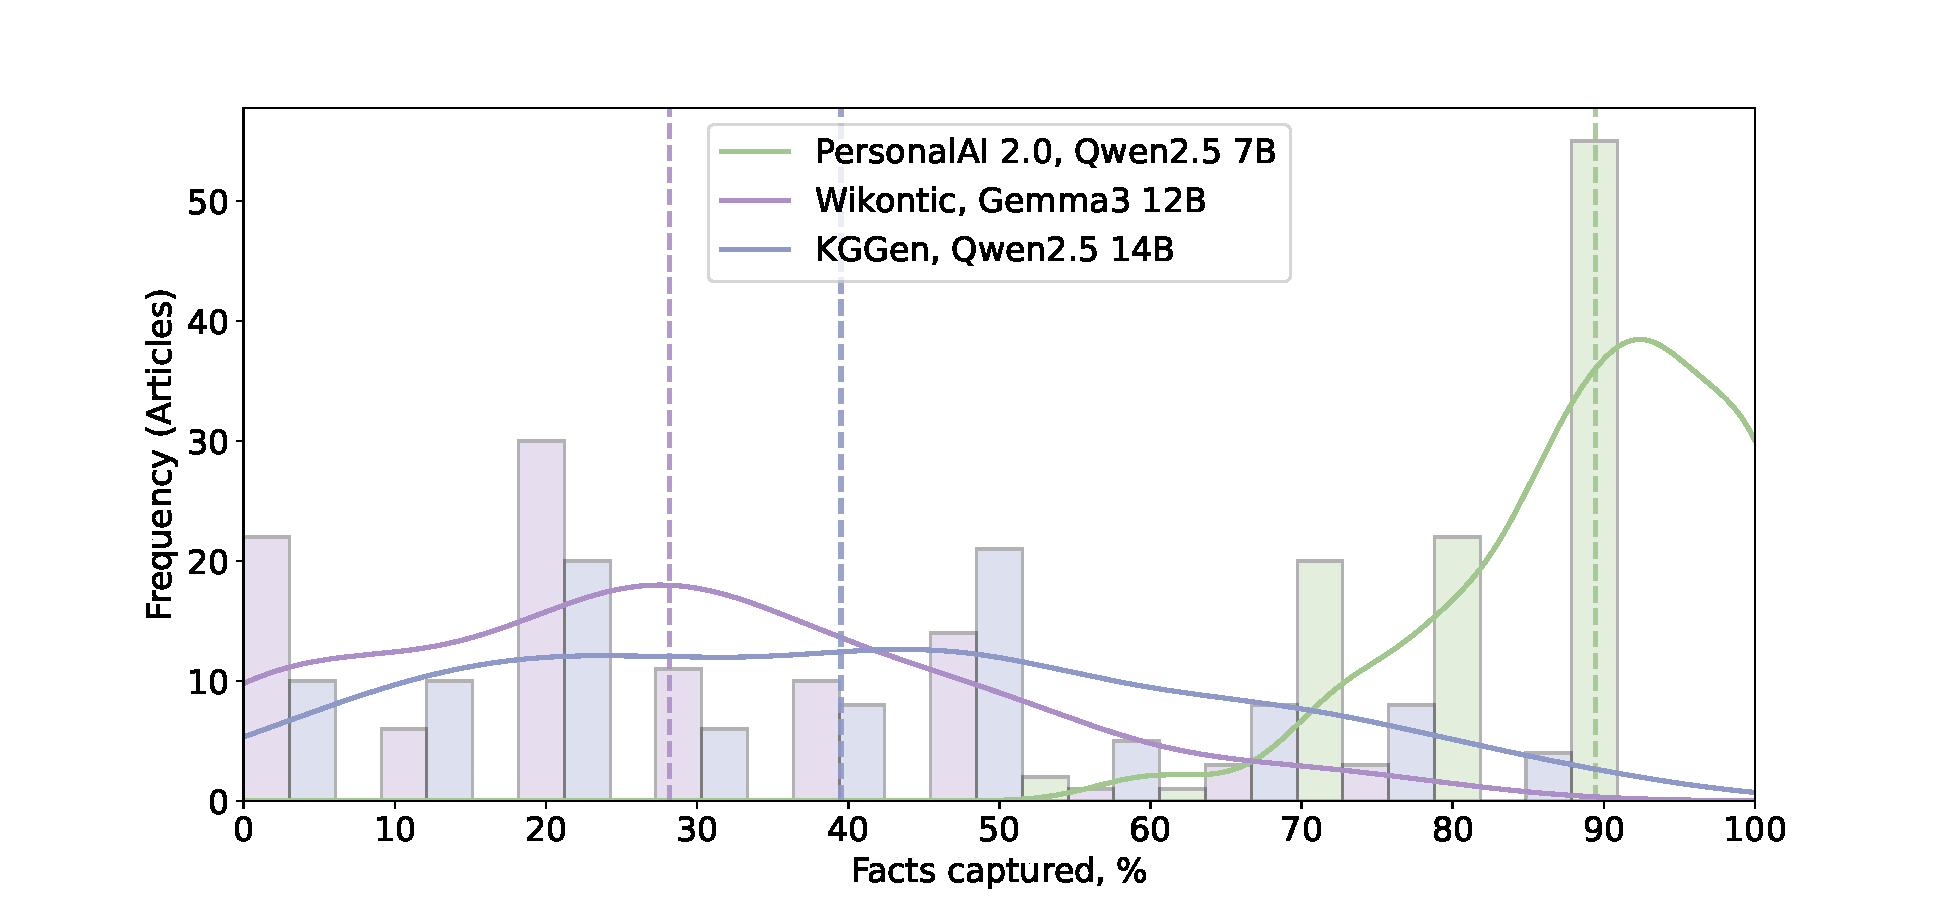
\includegraphics[width=.8\textwidth]{images/mine_pai_kgen_wikontic_comparison.pdf}
	\caption{Distribution of MINE-1 scores across 100 articles for PAI-2, Wikontic and KGGen. Dotted vertical lines are averaged scores. PAI-2 scored $89\%$ on average, substantially outperforming Wikontic $28\%$ and KGGen $39\%$.} 
	\label{fig:mine_diagram}
\end{figure}

We evaluated PAI-2 on the MINE-1 benchmark, which measures how much factual information from the source text is retained in the constructed KGs using an LLM-as-a-judge protocol from the original study~\cite{mo2025kggenextractingknowledgegraphs}. Figure~\ref{fig:mine_diagram} displays the retention scores distribution in articles of MINE-1 for PAI-2, Wikontick~\cite{chepurova-etal-2026-wikontic} and KGGen~\cite{mo2025kggenextractingknowledgegraphs}. Table ~\ref{tab:mine_comparison} demonstrates the results for KGGen~\cite{mo2025kggenextractingknowledgegraphs}, Wikontic~\cite{chepurova-etal-2026-wikontic}, GraphRAG~\cite{edge2025localglobalgraphrag} and PAI-2 with different LLM backbones. PAI-2 consistently outperforms other methods, reaching $89\%$ with Qwen2.5 7B, compared to Wikontick’s best score of $86\%$ (gpt4.1-mini). These results demonstrate that PAI effectively preserves factual information during the construction of memory graphs.

\begin{table}[H]
    \centering
	\renewcommand{\arraystretch}{1.3}
	%\resizebox{\textwidth}{!}{%
    \begin{tabular}{|c|c|c|}
    \hline
    \textbf{Method} & \textbf{LLM} & \textbf{MINE-1 Score (\%)} \\ \hline \hline
    \multirow{5}{*}{KGGen} & Claude Sonnet 3.5 & 73 \\ \cline{2-3} 
     & GPT-4o & 66 \\ \cline{2-3} 
     & Gemini 2.0 Flash & 44 \\ \cline{2-3} 
     & Qwen2.5 14B & 39 \\ \cline{2-3} 
     & Gemma3 12B & 14 \\ \hline
    \multirow{4}{*}{Wikontic} & gpt4.1-mini & 86 \\ \cline{2-3} 
     & gpt4o & 84 \\ \cline{2-3} 
     & Gemma3 12B & 28 \\ \cline{2-3} 
     & Qwen2.5 14B & 19 \\ \hline
    GraphRAG & gpt4o & 44 \\ \hline
    PAI-2 & Qwen2.5 7B & \textbf{89} \\ \hline
    \end{tabular}
    %}
    \caption{MINE-1 information-retention scores for KGGen, Wikontic, GraphRAG and PAI-2. PAI-2 achieves the highest retention performance across all evaluated LLMs. For PAI-2 evaluation, during triples retrieving (according to MINE setup) we only accept object and thesis vertices from constructed memory graph.}
	\label{tab:mine_comparison}
\end{table}

Additionally, we perform ablation experiments for PAI-2 to understand how MINE-1 score relates to LLM backbone and accepted vertex types: see Table~\ref{tab:mine_acceptedntypes_ablation}. This Table shows that the highest MINE-1 score is achieved when we accept triples, that is incident to all vertex types: object, thesis and episodic. However, when retrieving only episodic triples, quality degrades by only $1\%$. This means that object vertices (that are matched to the queries entities) are adjacent to episodic vertices, containing required knowledge to generate relevant responses. In other words, the set of object vertices, extracted from episodic memories, is sufficient to find a relevant, but redundant source document. Conversely, when generating responses based on triples, that incident only to object and thesis vertices, significant degradation is observed: on average 10\%. This may indicate that the number of thesis and simple triplets, extracted from episodic memories, is insufficient to cover the entire amount of knowledge they contain, which may be required to generate correct responses. Thus, to improve graph construction algorithm, it is necessary to include additional mechanics that : (1) evaluate the knowledge coverage degree of original document (episodic vertex) with corresponding set of extracted/generated triplets; (2) localize missing units of knowledge; (3) perform an additional extracting/generating round to get missing triples.

\begin{table}[H]
    \centering
	\renewcommand{\arraystretch}{1.3}
	%\resizebox{\textwidth}{!}{%
    \begin{tabular}{|c|c|c|c|c|c|c||c}
    \hhline{|-|------||-|}
    \multirow{2}{*}{\begin{tabular}[c]{@{}c@{}}\textbf{Accepted}\\ \textbf{Vertex Types}\end{tabular}} & \multicolumn{6}{c||}{\textbf{LLM}} & \multicolumn{1}{c|}{\multirow{2}{*}{Mean}} \\ 
    \hhline{|~|------||~|}
    & \multicolumn{1}{c|}{\textbf{Qwen2.5 7B}} & \multicolumn{1}{c|}{\textbf{Llama3.1 8B}} & \multicolumn{1}{c|}{\textbf{Granite3.3 8B}} & \multicolumn{1}{c|}{\textbf{Gemma2 9B}} & \multicolumn{1}{c|}{\textbf{Gemma3 12B}} & \textbf{Qwen2.5 14B} & \multicolumn{1}{c|}{} \\ 
    \hhline{=======::=}
    object & \cellcolor{lightsalmonpink} 67 & \cellcolor{lightsalmonpink} 38 & \cellcolor{lightsalmonpink} 52 & \cellcolor{lightsalmonpink} 61 & \cellcolor{lightsalmonpink} 77 & \cellcolor{lightsalmonpink} 64 & \multicolumn{1}{c|}{\cellcolor{lightsalmonpink} 60} \\ 
    \hhline{-------||-|}
    thesis & 81 & 76 & 66 & 81 & 76 & 80 & \multicolumn{1}{c|}{77} \\ 
    \hhline{-------||-|}
    episodic & 93 & \cellcolor{grannysmithapple} 94 & \cellcolor{grannysmithapple} 95 & 94 & 93 & 93 & \multicolumn{1}{c|}{94} \\ 
    \hhline{-------||-|}
    object, thesis & 89 & 80 & 78 & 89 & 85 & 88 & \multicolumn{1}{c|}{85} \\ 
    \hhline{-------||-|}
    object, thesis, episodic & \cellcolor{grannysmithapple} 96 & \cellcolor{grannysmithapple} 94 & 94 & \cellcolor{grannysmithapple} 96 & \cellcolor{grannysmithapple} 97 & \cellcolor{grannysmithapple} 95 & \multicolumn{1}{c|}{\cellcolor{grannysmithapple} 95} \\
    \hhline{=======::=}
    Mean & 85 & \cellcolor{lightsalmonpink} 76 & 77 & 84 & \cellcolor{grannysmithapple} 86 & 84 & \multicolumn{1}{c|}{82} \\
    \hhline{|-|------||-|}
    \end{tabular}%}
    \renewcommand{\arraystretch}{1}
    \caption{Dependence of MINE-1 information-retention score on accepted vertex types for PAI 2.0 across six LLMs.}
	\label{tab:mine_acceptedntypes_ablation}
\end{table}

% TODO


\section{Human Evaluation}
\label{app:human_evaluation}

Krippendorff’s alpha and Pearson correlation coefficients, calculated for each best PAI-2 and HippoRAG 2 experiment setup can be seen in Tables~\ref{tab:humaneval_kripalpha} and~\ref{tab:humaneval_pearsoncoef} correspondingly. Comparison of human and Judge (Qwen2.5 7B) evaluation can be seen in Figure~\ref{tab:humaneval_vs_judgescores}.

\begin{table}[H]
    \centering
	\renewcommand{\arraystretch}{1.3}
	%\resizebox{\textwidth}{!}{%
    \begin{tabular}{|c|c|c|c|c|c|c||c|}
    \hhline{|-------||-|}
    \multirow{2}{*}{\textbf{Method}} & \multicolumn{6}{c||}{\textbf{Dataset}} & \multirow{2}{*}{Mean} \\ \hhline{|~|------||~|}
     & \textbf{Natural Questions} & \textbf{TriviaQA} & \textbf{HotpotQA} & \textbf{2WikiMultihopQA} & \textbf{MuSiQue} & \textbf{DiaASQ} &  \\ 
    \hhline{|=======::=}
    HippoRAG 2 & 0.92 & 0.92 & 0.92 & 0.92 & 0.97 & 0.97 & 0.94 \\ 
    \hhline{|-------||-|}
    PAI-2 & 0.86 & 0.95 & 0.95 & 0.95 & 0.91 & 0.97 & 0.93 \\ 
    \hhline{|-------||-|}
    \end{tabular}%}
    \renewcommand{\arraystretch}{1}
    \caption{Krippendorff’s alpha coefficients of HumanEval scores, calculated for best HippoRAG 2 and PAI-2 configurations across six datasets}
	\label{tab:humaneval_kripalpha}
\end{table}

\begin{table}[H]
    \centering
	\renewcommand{\arraystretch}{1.3}
	%\resizebox{\textwidth}{!}{%
    \begin{tabular}{|c|c|c|c|c|c|c||c|}
    \hhline{|-------||-|}
    \multirow{2}{*}{\textbf{Method}} & \multicolumn{6}{c||}{\textbf{Dataset}} & \multirow{2}{*}{Mean} \\ \hhline{|~|------||~|}
     & \textbf{Natural Questions} & \textbf{TriviaQA} & \textbf{HotpotQA} & \textbf{2WikiMultihopQA} & \textbf{MuSiQue} & \textbf{DiaASQ} &  \\ 
    \hhline{|=======::=}
    HippoRAG 2 & 0.76 & 0.94 & 0.85 & 0.85 & 0.82 & 0.84 & 0.84 \\
    \hhline{|-------||-|}
    PAI-2 & 0.84 & 0.92 & 0.85 & 0.96 & 0.80 & 0.95 & 0.88 \\
    \hhline{|-------||-|}
    \end{tabular}%}
    \renewcommand{\arraystretch}{1}
    \caption{Pearson correlation coefficients between LLM-as-a-Judge and HumanEval scores, calculated for HippoRAG 2 and PAI-2 best configurations across six datasets}
	\label{tab:humaneval_pearsoncoef}
\end{table}

\begin{table}[H]
    \centering
	\renewcommand{\arraystretch}{1.3}
	%\resizebox{\textwidth}{!}{%
    \begin{tabular}{|c|c|c|c|c|c|c|c||c|}
    \hhline{|-|-|------||-|}
    \multirow{2}{*}{\textbf{Method}} & \multirow{2}{*}{\textbf{Metric}} & \multicolumn{6}{c||}{\textbf{Dataset}} & \multirow{2}{*}{Mean} \\ 
    \hhline{|~|~|------||~|}
     &  & \textbf{Natural Questions} & \textbf{TriviaQA} & \textbf{HotpotQA} & \textbf{2WikiMultihopQA} & \textbf{MuSiQue} & \textbf{DiaASQ} &  \\ 
    \hhline{========::=}
    \multirow{2}{*}{HippoRAG 2} & HumanEval & 0.83 & 0.78 & 0.75 & 0.54 & 0.33 & 0.34 & 0.60 \\
    \hhline{|~|-|-|-|-|-|-|-||-|}
     & LLM-as-a-Judge & 0.80 & 0.77 & 0.73 & 0.56 & 0.29 & 0.28 & 0.57 \\
     \hhline{========:|=}
    \multirow{2}{*}{PAI-2} & HumanEval & 0.68 & 0.80 & 0.73 & 0.57 & 0.36 & 0.35 & 0.58 \\ \hhline{|~|-|-|-|-|-|-|-||-|}
     & LLM-as-a-Judge & 0.69 & 0.80 & 0.67 & 0.58 & 0.33 & 0.34 & 0.56 \\ 
     \hhline{|-|-|-|-|-|-|-|-||-|}
    \end{tabular}%}
    \renewcommand{\arraystretch}{1}
    \caption{HumanEval and LLM-as-a-Judge scores for HippoRAG 2 and PAI-2 best configurations across six datasets}
	\label{tab:humaneval_vs_judgescores}
\end{table}

Annotation was conducted by the three authors of the work, so no additional recruitment or payment are required on this stage. All assessors held bachelor’s degrees and had prior experience in the evaluation of LLM responses.

% \section{Comparison of PersonalAI`s QA pipeline with and w/o use of elements relations in constructed knowledge graph}
% \label{app:nr_vs_gt_comparison}

% \definecolor{grannysmithapple}{rgb}{0.66, 0.89, 0.63}
% \definecolor{lightsalmonpink}{rgb}{1.0, 0.6, 0.6}

% \begin{table}[H]
%     \centering
% 	\renewcommand{\arraystretch}{1.3}
% 	\resizebox{\textwidth}{!}{%
%     \begin{tabular}{|c|c|c|c|c|c|c|c|c||c|}
%     \hhline{|-|-|-|------||-}
%     \multicolumn{1}{|c|}{\multirow{2}{*}{\textbf{Method}}} & \multicolumn{1}{c|}{\multirow{2}{*}{\begin{tabular}[c]{@{}c@{}}\textbf{Accepted} \\ \textbf{Triplet Types}\end{tabular}}} & \multirow{2}{*}{\textbf{LLM}} & \multicolumn{6}{c||}{\textbf{Dataset}} & \multirow{2}{*}{Mean} \\ 
%     \hhline{|~|~|~|------||~|}
%     \multicolumn{1}{|c|}{} & \multicolumn{1}{c|}{} &  & \textbf{Natural Questions} & \textbf{TriviaQA} & \textbf{HotpotQA} & \textbf{2WikiMultihopQA} & \textbf{MuSiQue} & \textbf{DiaASQ} &  \\ 
%     \hhline{=========:|-|}
%     \multicolumn{1}{|c|}{\multirow{4}{*}{PersonalAI 1.0}} & \multicolumn{1}{c|}{simple} & \multirow{8}{*}{Qwen2.5 7B} & 0.63 / 0.62 / 0.47 & 0.63 / 0.66 / 0.68 & 0.63 / 0.45 / 0.48 & - / - / 0.26 & \cellcolor{grannysmithapple} 0.23 / 0.52 / \textbf{0.13} & \cellcolor{lightsalmonpink} - / - / 0.07 & 0.53 / 0.56 / 0.35 \\ 
%     \hhline{|~|-|~|-|-|-|-|-|-||-|}
%     \multicolumn{1}{|c|}{} & \multicolumn{1}{c|}{hyper} &  & 0.60 / 0.57 / 0.45 & 0.63 / 0.69 / 0.64 & - / - / 0.35 & - / - / 0.23 & \cellcolor{lightsalmonpink} 0.21 / \textbf{0.68} / 0.06 & \cellcolor{grannysmithapple} - / - / \textbf{0.15} & 0.48 / \textbf{0.65} / 0.31 \\ 
%     \hhline{|~|-|~|-|-|-|-|-|-||-|}
%     \multicolumn{1}{|c|}{} & \multicolumn{1}{c|}{simple, hyper} &  & \cellcolor{grannysmithapple} \textbf{0.68} / \textbf{0.64} / \textbf{0.56} & \cellcolor{grannysmithapple}\textbf{0.68} / \textbf{0.74} / \textbf{0.70} & \cellcolor{grannysmithapple} \textbf{0.65} / \textbf{0.62} / \textbf{0.50} & \cellcolor{grannysmithapple} - / - / \textbf{0.29} & \textbf{0.32} / 0.46 / 0.12 & - / - / 0.14 & \cellcolor{grannysmithapple} \textbf{0.58} / 0.62 / \textbf{0.38} \\ 
%     \hhline{|~|-|~|-|-|-|-|-|-||-|}
%     \multicolumn{1}{|c|}{} & \multicolumn{1}{c|}{episodic} &  &  \cellcolor{lightsalmonpink} 0.48 / 0.61 / 0.37 &  \cellcolor{lightsalmonpink} 0.65 / \textbf{0.74} / 0.44 & \cellcolor{lightsalmonpink} - / - / 0.21 & \cellcolor{lightsalmonpink} 0.41 / 0.51 / 0.13 & 0.16 / 0.56 / - & - / - / - & \cellcolor{lightsalmonpink} 0.42 / 0.60 / 0.29 \\ 
%     \hhline{==|~|======::=}
%     \multicolumn{1}{|c|}{\multirow{4}{*}{PersonalAI 2.0}} & \multicolumn{1}{c|}{simple} &  & \cellcolor{lightsalmonpink} 0.86 / \textbf{0.96} / 0.58 & 0.86 / 0.87 / 0.69 & \textbf{0.83} / \textbf{0.85} / 0.59 & 0.59 / 0.67 / \textbf{0.48} & \cellcolor{lightsalmonpink} \textbf{0.69} / \textbf{0.86} / 0.25 & 0.49 / 0.56 / 0.10 & 0.72 / 0.80 / 0.45 \\ 
%     \hhline{|~|-|~|-|-|-|-|-|-||-|}
%     \multicolumn{1}{|c|}{} & \multicolumn{1}{c|}{hyper} &  & \textbf{0.90} / 0.92 / 0.59 & 0.88 / 0.86 / 0.72 & \cellcolor{lightsalmonpink} 0.73 / 0.79 / 0.50 & 0.52 / 0.74 / 0.34 & 0.59 / 0.73 / 0.27 & 0.62 / 0.61 / 0.25 & 0.71 / 0.78 / 0.44 \\ 
%     \hhline{|~|-|~|-|-|-|-|-|-||-|}
%     \multicolumn{1}{|c|}{} & \multicolumn{1}{c|}{simple, hyper} &  & 0.88 / \cellcolor{grannysmithapple}  \textbf{0.96} / \textbf{0.64} & \cellcolor{grannysmithapple} \textbf{0.89} / \textbf{0.88} / \textbf{0.77} & \cellcolor{grannysmithapple} 0.82 / \textbf{0.85} / \textbf{0.63} & \cellcolor{grannysmithapple} \textbf{0.60} / \textbf{0.78} / \textbf{0.48} & 0.68 / \textbf{0.86} / 0.28 & \cellcolor{grannysmithapple} \textbf{0.66} / 0.60 / \textbf{0.26} & \cellcolor{grannysmithapple} \textbf{0.76} / \textbf{0.82} / \textbf{0.51} \\ 
%     \hhline{|~|-|~|-|-|-|-|-|-||-|}
%     \multicolumn{1}{|c|}{} & \multicolumn{1}{c|}{episodic} &  & 0.75 / 0.93 / 0.60 & \cellcolor{lightsalmonpink} - / - / 0.66 & 0.73 / 0.81 / 0.55 & \cellcolor{lightsalmonpink} 0.48 / 0.75 / 0.33 & \cellcolor{grannysmithapple} 0.62 / 0.82 / \textbf{0.32} & \cellcolor{lightsalmonpink} 0.32 / \textbf{0.62} / 0.06 & \cellcolor{lightsalmonpink} 0.58 / 0.79 / 0.42 \\ 
%     \hhline{=========::=}
%     \multicolumn{3}{|c|}{Mean (PersonalAI 1.0)} & 0.60 / 0.61 / 0.46 & 0.65 / 0.71 / 0.62 & 0.64 / 0.54 / 0.38 & 0.41 / 0.51 / 0.23 & 0.23 / 0.56 / 0.10 & - & 0.51 / 0.60 / 0.34 \\ 
%     \hhline{|---|-|-|-|-|-|-||-|}
%     \multicolumn{3}{|c|}{Mean (PersonalAI 2.0)} & 0.85 / 0.94 / 0.60 & 0.88 / 0.87 / 0.71 & 0.78 / 0.82 / 0.57 & 0.55 / 0.74 / 0.41 & 0.64 / 0.82 / 0.28 & 0.52 / 0.60 / 0.17 & 0.70 / 0.79 / 0.46 \\
%     \hhline{|---|-|-|-|-|-|-||-|}
%     \end{tabular}}
%     \renewcommand{\arraystretch}{1}
%     \caption{Dependence of PAI 1.0 and PAI 2.0 performance on accepted triples types for final answer generation across six datasets. For graph/triples traversal/retrieval NaiveRetriever algorithm is set}
% 	\label{tab:nr_vs_gt_comparison}
% \end{table}

% TODO

% \section{LLM, graph traversal and according restriction selection}
% \label{app:hyperp_selection}
% % TODO

% \section{Query preprocessing Ablation}
% \label{app:query_preprocessing}
% % TODO

